\documentclass[pdftex,a4paper,14pt,english,russian]{extarticle}

\usepackage[top=2cm,bottom=27mm,left=3cm,right=18mm]{geometry}
\usepackage[T2A]{fontenc}
\usepackage[utf8]{inputenc}
\usepackage[english,russian]{babel}
\usepackage[pdftex]{hyperref}
\usepackage{indentfirst}
\usepackage[pdftex]{graphicx}
\usepackage{amsmath}
\usepackage{amssymb}
\newcommand*\Laplace{\mathop{}\!\mathbin\bigtriangleup}
\usepackage[makeroom]{cancel}
\usepackage{ragged2e}

\usepackage{multirow}
\usepackage{algorithmic}
\usepackage[boxed]{algorithm}
\usepackage{tabularx}
\usepackage{xtab}
\usepackage{subfig}
\usepackage{hyphenat}
\usepackage{setspace}
\usepackage{fancyhdr}

\usepackage[usenames, dvipsnames]{color}
\definecolor{mygreen}{rgb}{0,0.6,0}
\usepackage{listings}
 \lstset{commentstyle=\color{mygreen},
 literate=
 	{~}{{\textasciitilde}}1
 	{а}{{\selectfont\char224}}1
 	{б}{{\selectfont\char225}}1
 	{в}{{\selectfont\char226}}1
 	{г}{{\selectfont\char227}}1
 	{д}{{\selectfont\char228}}1
 	{е}{{\selectfont\char229}}1
 	{ё}{{\"e}}1
 	{ж}{{\selectfont\char230}}1
 	{з}{{\selectfont\char231}}1
 	{и}{{\selectfont\char232}}1
 	{й}{{\selectfont\char233}}1
 	{к}{{\selectfont\char234}}1
 	{л}{{\selectfont\char235}}1
 	{м}{{\selectfont\char236}}1
 	{н}{{\selectfont\char237}}1
 	{о}{{\selectfont\char238}}1
 	{п}{{\selectfont\char239}}1
 	{р}{{\selectfont\char240}}1
 	{с}{{\selectfont\char241}}1
 	{т}{{\selectfont\char242}}1
 	{у}{{\selectfont\char243}}1
 	{ф}{{\selectfont\char244}}1
 	{х}{{\selectfont\char245}}1
 	{ц}{{\selectfont\char246}}1
 	{ч}{{\selectfont\char247}}1
 	{ш}{{\selectfont\char248}}1
 	{щ}{{\selectfont\char249}}1
 	{ъ}{{\selectfont\char250}}1
 	{ы}{{\selectfont\char251}}1
 	{ь}{{\selectfont\char252}}1
 	{э}{{\selectfont\char253}}1
 	{ю}{{\selectfont\char254}}1
 	{я}{{\selectfont\char255}}1
 	{А}{{\selectfont\char192}}1
 	{Б}{{\selectfont\char193}}1
 	{В}{{\selectfont\char194}}1
 	{Г}{{\selectfont\char195}}1
 	{Д}{{\selectfont\char196}}1
 	{Е}{{\selectfont\char197}}1
 	{Ё}{{\"E}}1
 	{Ж}{{\selectfont\char198}}1
 	{З}{{\selectfont\char199}}1
 	{И}{{\selectfont\char200}}1
 	{Й}{{\selectfont\char201}}1
 	{К}{{\selectfont\char202}}1
 	{Л}{{\selectfont\char203}}1
 	{М}{{\selectfont\char204}}1
 	{Н}{{\selectfont\char205}}1
 	{О}{{\selectfont\char206}}1
 	{П}{{\selectfont\char207}}1
 	{Р}{{\selectfont\char208}}1
 	{С}{{\selectfont\char209}}1
 	{Т}{{\selectfont\char210}}1
 	{У}{{\selectfont\char211}}1
 	{Ф}{{\selectfont\char212}}1
 	{Х}{{\selectfont\char213}}1
 	{Ц}{{\selectfont\char214}}1
 	{Ч}{{\selectfont\char215}}1
 	{Ш}{{\selectfont\char216}}1
 	{Щ}{{\selectfont\char217}}1
 	{Ъ}{{\selectfont\char218}}1
 	{Ы}{{\selectfont\char219}}1
 	{Ь}{{\selectfont\char220}}1
 	{Э}{{\selectfont\char221}}1
 	{Ю}{{\selectfont\char222}}1
 	{Я}{{\selectfont\char223}}1
 	{і}{{\selectfont\char105}}1
 	{ї}{{\selectfont\char168}}1
 	{є}{{\selectfont\char185}}1
 	{ґ}{{\selectfont\char160}}1
 	{І}{{\selectfont\char73}}1
 	{Ї}{{\selectfont\char136}}1
 	{Є}{{\selectfont\char153}}1
 	{Ґ}{{\selectfont\char128}}1
}
\newcommand{\angstrom}{\buildrel _{\circ} \over {\mathrm{A}}}
\numberwithin{equation}{subsection}
\pagestyle{fancyplain}
\fancyhf{}
\renewcommand{\headrulewidth}{0pt}
\rfoot{\fancyplain{}{\thepage}}

\linespread{1.15}
\floatname{algorithm}{Алгоритм}

\addto\captionsrussian{  \renewcommand{\contentsname}{СОДЕРЖАНИЕ}}
\addto\captionsrussian{ \renewcommand\refname{СПИСОК ИСПОЛЬЗОВАННЫХ ИСТОЧНИКОВ}}
% прилоение
\addto\captionsrussian{ \renewcommand\appendixname{ПРИЛОЖЕНИЕ}}
\makeatletter
\def\redeflsection{\def\l@section{\@dottedtocline{1}{1.5em}{7.8em}}}
\renewcommand\appendix{\par
\setcounter{section}{0}%
\setcounter{subsection}{0}%
\def\@chapapp{\appendixname}%
\addtocontents{toc}{\protect\redeflsection}
\def\thesection{\appendixname\hspace{0.2cm}\@arabic\c@section}}
\makeatother
% /прилоение
% new commands
\newcommand\sign[1]{sign(#1)}

\begin{document}

\begin{titlepage}
  \begin{center}
    % \textsc{\small Министерство образования Республики Беларусь}\\[0.5cm]
    \textsc{\small \large федеральное государственное бюджетное образовательное
    учреждение высшего образования "московский государственный университет им. Ломоносова"}\\[0.3cm]
    \textsc{\large Физический факультет}\\[0.3cm]
    \textsc{\large кафедра оптики, спектроскопии и физики наносистем}\\[0.5cm]

    \begin{minipage}{\textwidth}
      \begin{flushleft}

      \end{flushleft}
    \end{minipage}\\[0.5cm]

    \textsc{\large  магистерская диссертация}\\[0.5cm]
    \textbf{\large Двух- и трехкристальная дифрактометрия в исследовании
    пьезоэлектрических кристаллов в условиях воздействия электрического поля}\\[1.5cm]


    \begin{minipage}{\textwidth}
      \begin{flushright}
        Выполнил студент группы 241М \hspace*{2.1cm} \\
        Аткнин И. И.\underline{\hspace*{4.6cm}}\\[0.5cm]
        Научный руководитель: к.ф.-м. н. \hspace*{1.8cm} \\
        Марченков Н. В. \underline{\hspace*{3.7cm}}\\[0.5cm]
        Научный руководитель: к.ф.-м. н., доцент\\
        Стремоухов С. Ю. \underline{\hspace*{3.7cm}}\\[0.5cm]
      \end{flushright}
    \end{minipage}\\[1.5cm]


    \begin{minipage}{\textwidth}
      \begin{flushleft}
        \textit{Допущена к защите 31.05.2017}\\
        Зав. кафедрой \underline{\hspace*{4.5cm}}\\
      \end{flushleft}
    \end{minipage}\\[1.5cm]

    \vfill
    \textsc{\small Москва\\ 2017}
  \end{center}
\end{titlepage}


\setcounter{page}{5}
\begin{center}
\tableofcontents
\end{center}

% \tableofcontents
\newpage


\section{Литературный обзор}

Рентгеновское излучение, взаимодействуя с электронами атомов вещества рассеивается.
Протоны (ядра атомов) в рассеянии рентгеновских лучей практически не участвуют, т.к.
амплитуда электромагнитной волны, рассеянной заряженной частицей,
 обратно пропорциональна ее массе - формула Томсона \cite{iveronova1972}. Величина такого рассеяния
 зависит от количества электронов в атоме.  Тяжелые металлы,
 например свинец, Pb (Z = 82), рассеивают рентгеновское излучение сильнее легких,
 таких как Ni (Z = 28) или  Co (Z = 27), а такие атомы, как He или H – прозрачны
 для рентгеновского излучения.  Атомный множитель $f$ (атомный фактор рассеяния) определяется
как отношение амплитуды волны, рассеянной одним атомом, к амплитуде волны, рассеянной
одним свободным электроном. Действительно, если в какой либо точке пространства сосредоточено
$Z$ электронов, то заряд этой группы равен $Q = Z\cdot e$, а масса $M = Z \cdot m_e$.

На рис. \ref{ris:atom_factor} представлена диаграмма направленности атомного
фактора лантана в зависимости от угла. Размеры атома соизмеримы с длиной волны
рентгеновских лучей, поэтому между волнами рассеянными отдельными электронами, возникает
разность фаз. Это разность фаз равна нулю только при $2 \theta = 0$, поэтому структурный
фактор зависит от $\theta$ и $\lambda$. Максимальная величина, которая равна $Z$,
 наблюдается в случае рассеяния вперед.

\begin{figure}[H]
  \centering
  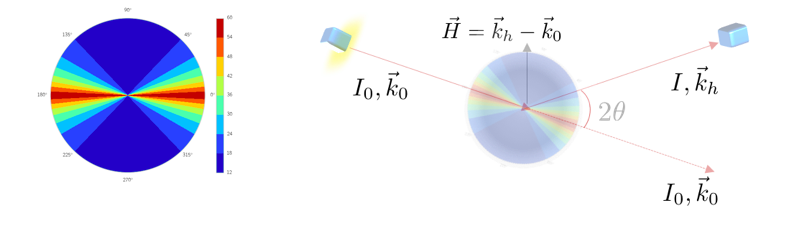
\includegraphics[width=0.9\textwidth]{images/atom_factor.png}
  \caption{ (Слева) фактор рассеяния для атома лантана (La, N = 57), (справа)
  схема расположения векторов для падающей и рассеянной волн}
  \label{ris:atom_factor}
\end{figure}

Приближенное выражение для расчета атомного фактора рассеяния
представляется \cite{International_Tables} в виде выражения:

\begin{equation}
  f_0 = \sum_{i=1}^{4} \cdot a_i e^{ -b_i (\frac{sin \vartheta_B}{\lambda})^2} + C
 \end{equation}
где $a_i$, $b_i$ и $c$ - коэффициенты Кромер-Манна для бездисперсионного канала рассеяния атомами решетки,
ограничением является $0<\frac{sin\vartheta}{\lambda}<2.0 \angstrom ^{-1}$.
 Характерная зависимость структурного фактора от угла рассеяния и длины волны
для атомов входящих в состав кристалла LGT (La, Ga, Ta, O) представлена на рис. \ref{ris:atom_factor_GaLaTa}.

\begin{figure}[H]
  \centering
  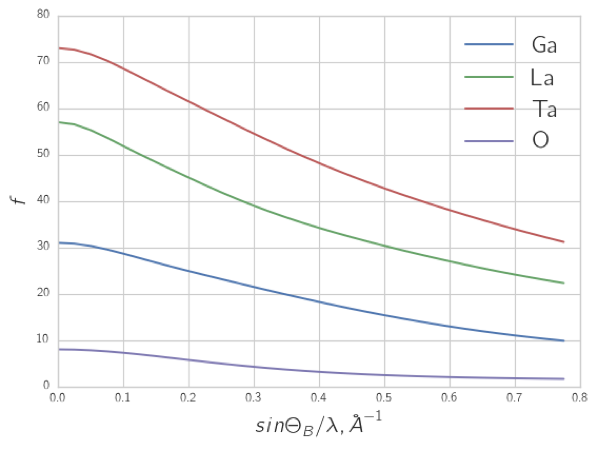
\includegraphics[width=0.6\textwidth]{images/atom_factor_GaLaTa.png}
  \caption{ Атомный фактор рассеяния для атомов: галлия (Ga), лантана (La), тантала (Ta) и  кислорода (O)}
  \label{ris:atom_factor_GaLaTa}
\end{figure}

При расчете интенсивности рассеяния атомом необходимо учитывать факт,
что все электроны связаны между собой, таким образом необходимо записывать
уравнение движение связанного электрона по действием падающего излучения.
Если атом многоэлектронный, то амплитуда рассеянной волны равна сумме амплитуд волн,
рассеянных всеми электронами атома, в результате структурный фактор \cite{iveronova1972}:

\begin{equation}
  f = f_0 + f^{'} + i f^{''}
 \end{equation}
\noindent
где, $f_0$ - атомный фактор рассеяния, рассчитанный без учета сил связи электронов
 с ядром, а $f^{'}$ и $f^{''}$ - дисперсионные поправки \cite{f0f1f12},
 первая из которых учитывает дополнительное рассеяние,
а вторая - дополнительное поглощение вблизи собственных частот колебаний электронов в атоме.

 \begin{figure}[H]
   \centering
   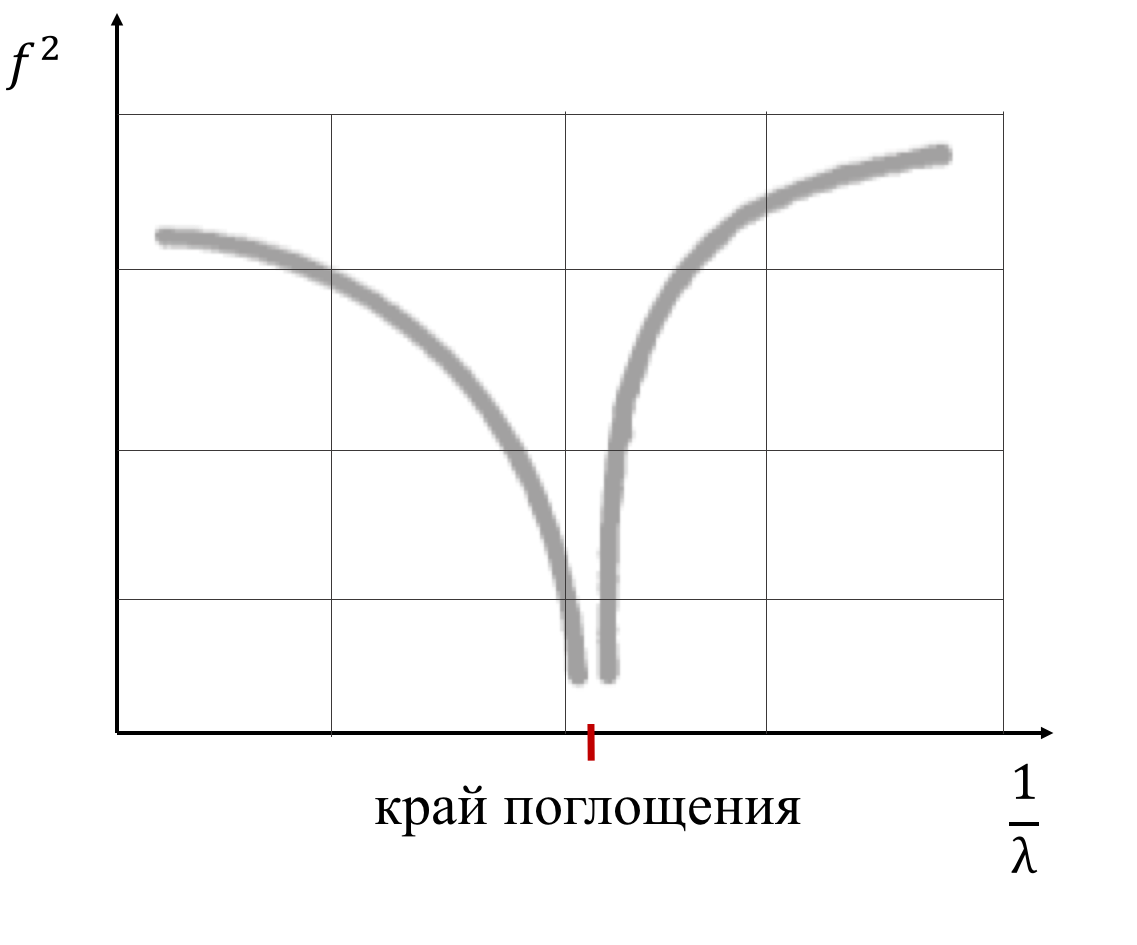
\includegraphics[width=0.4\textwidth]{images/dispers_f.png}
   \caption{ Схематичная зависимость квадрата атомного фактора $f^2 = (f_0 + f^{'})^2 + (f^{''})^2 $ от
   длины волны $\lambda$ вблизи края поглощения}
   \label{ris:dispers_f}
 \end{figure}

Важной особенностью является факт того, что дисперсионные поправки $f^{'}$, $f^{''}$
практически не зависят от длины волны, но зависят от энергии. Так как $f_0$ уменьшается
с ростом угла рассеяния, дисперсионные поправки начинают играть роль при больших углах $\theta$.

\label{sec:structure_factor}
Атомы решетки, взаимодействуя с рентгеновским излучением, рассеивают его.
Если в элементарной ячейке более одного атома, волны от разных атомов,
 интерферируя между собой, вносят вклад в общую картину рассеяния,
 ослабляя или усиливая ее.

 \begin{figure}[H]
   \centering
   \subfloat[]{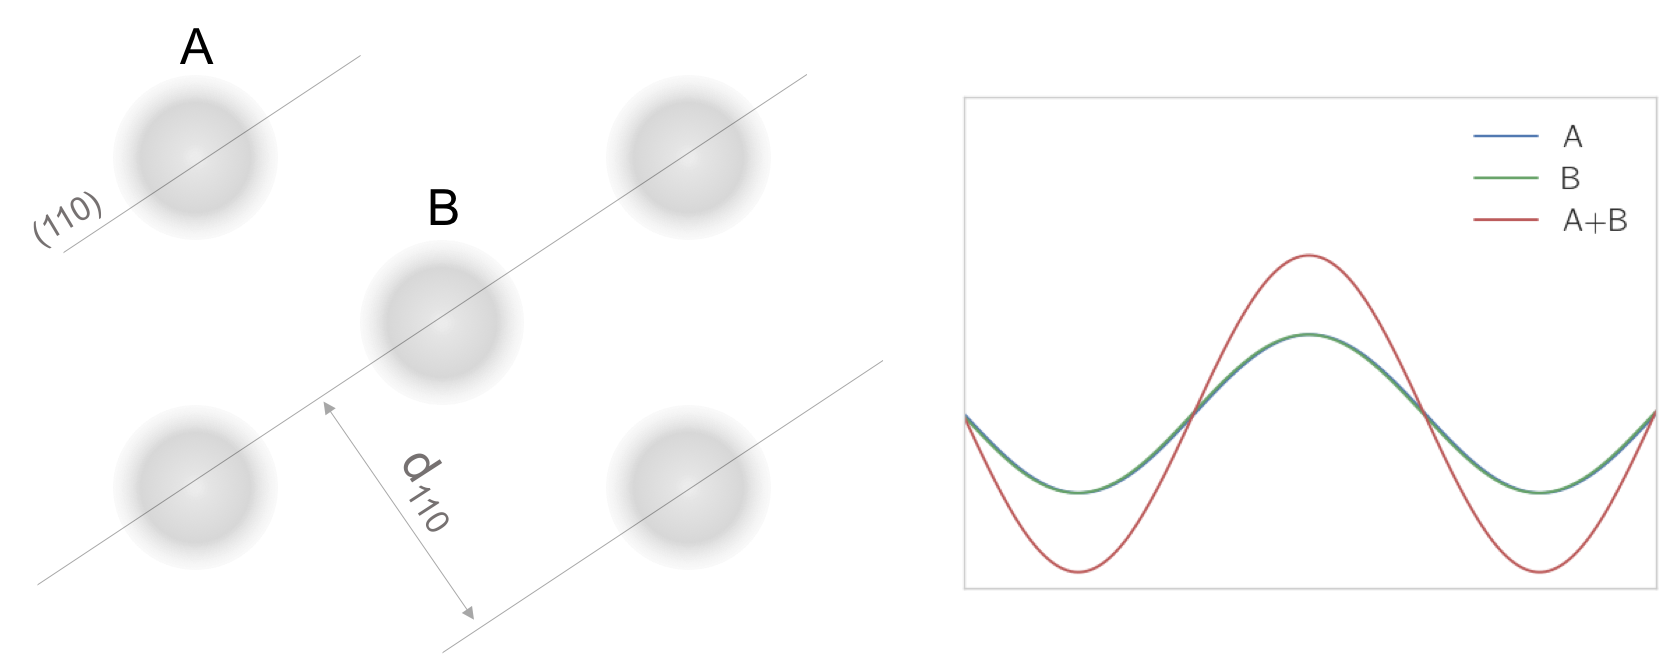
\includegraphics[width=0.45\textwidth]{images/interference_construct.png}}
   \hfill
   \subfloat[]{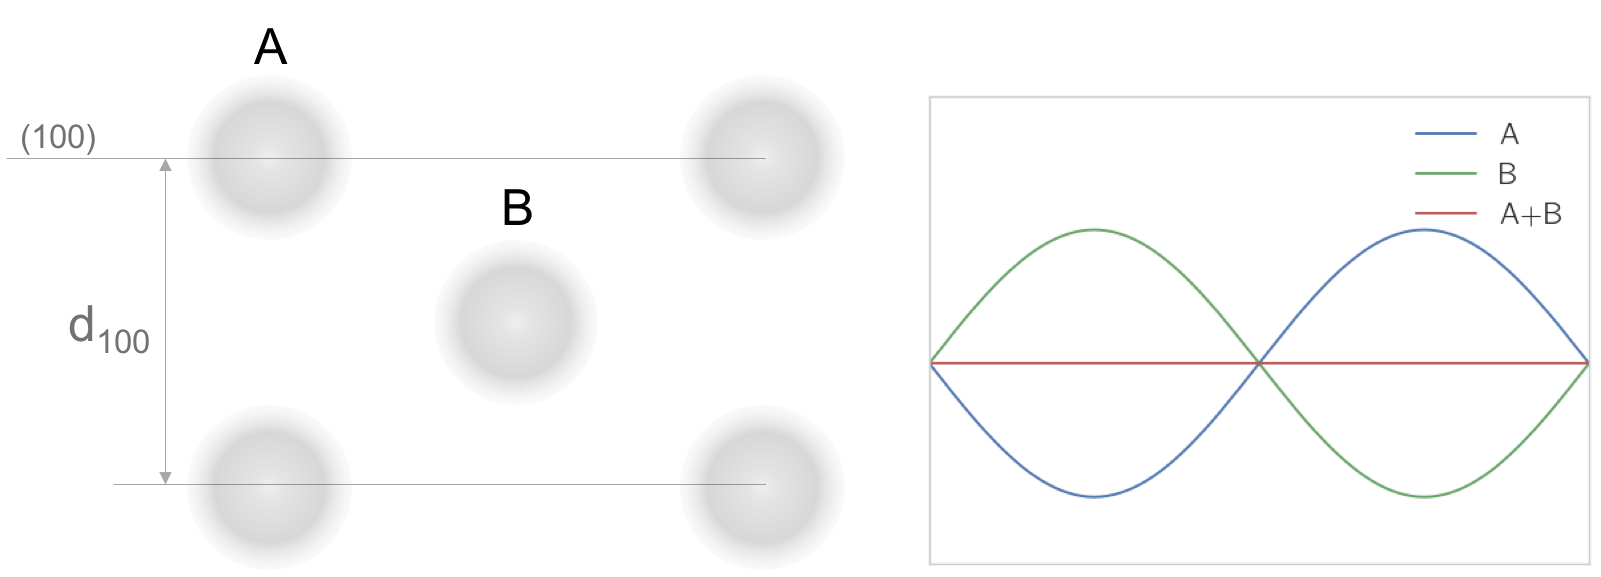
\includegraphics[width=0.45\textwidth]{images/interference_destruct.png}}
   \caption{Примеры интерференции двух волн, отраженных различными системами атомных плоскостей для случая
   конструктивной (a) и деструктивной (b) интерференции}
   \label{ris:interference_by_plate}
 \end{figure}

Рассеяние от набора атомов характеризуется структурным фактором, определяемым векторным
 сложением фаз по всем N атомам элементарной ячейки:

 \begin{equation}
   F = \sum_{n} f_n e^{ i\vec{h}\vec{r}_n} =   \sum_{n} f_n \cdot e^{-i\phi_n},
   \label{eq:F_factor}
  \end{equation}
\noindent
где $\phi_n = 2 \pi (hx_n+ky_n+lz_n)$;  $h, k, l$ - индексы Миллера; $x, y, z$ - относительные координаты
атомов в элементарной ячейке.

В соответсвии с \ref{eq:F_factor} в качестве примера был произведен расчет трехмерной ($hkl$) -
карты струкутрного фактора (рис. \ref{ris:hkl_LGT_SI}).
Цветом изображена величина структурного фактора для разных
 индексов плоскостей отражения для кристаллов LGT и Si.
 В таком представлении просматривается периодичность образования запрещенных
 рефлексов в кубическом кремнии. В кристалле LGT запрещенных (синий цвет)
  индексов для отражения на порядок меньше, связанно это с более низкой
  симметрией кристалла.

  \begin{figure}[h]
    \centering
    \subfloat[]{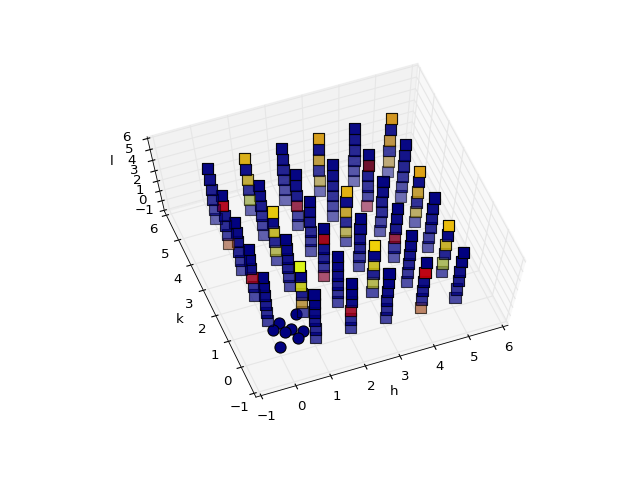
\includegraphics[width=0.5\textwidth]{images/hkl_Si.png} \label{ris:hkl_LGT_SI_a}}
    \hfill
    \subfloat[]{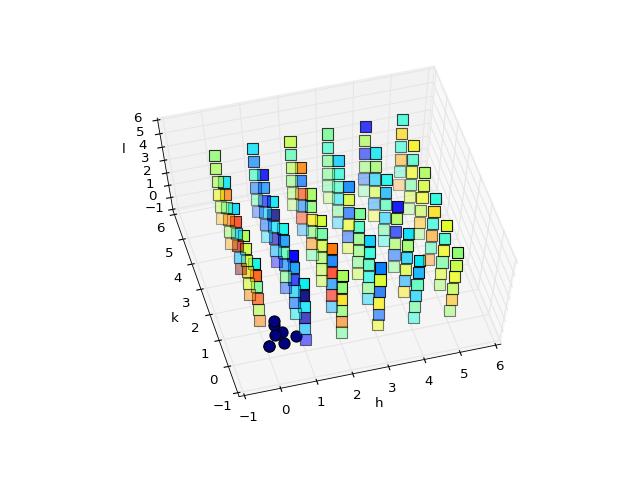
\includegraphics[width=0.5\textwidth]{images/hkl_LGT.png} \label{ris:hkl_LGT_SI_b}}
    \caption{Карта распределения величины структурного фактора
    (цвет соответствует его величине) в координатах индексов Миллера для кристалла Si (a) и LGT (b)}
    \label{ris:hkl_LGT_SI}
  \end{figure}

\subsection{Влияние температуры. Тепловой фактор}

При расчете структурных амплитуд рассеяния необходимо учитывать
тепловые колебания атомов в решетке. Предположим, что атомы колеблется около положения
равновесия независимо друг от друга, тогда это эквивалентно увеличения радиуса атома,
что приводит к более быстрому спаду функции атомного рассеяния с ростом угла рассеяния.
С другой стороны эффективное увеличение радиуса атома, очевидно должно зависеть от
величины среднеквадратичного смещения смещения атома  $<u^2>$ из положения равновесия.
Также для простоты предположим, что период тепловых колебаний атомов намного больше периода
колебаний падающего излучения, тем самым мы можем считать атом неподвижным в момент рассеяния,
т.е. пренебречь эффектом Доплера.

Таким образом структурный фактор необходимо усреднить за время наблюдения по всем возможным отклонениям
\begin{equation}
  F_T = \left\langle \sum_{n} f_n \cdot  e^{-i\vec {h} \cdot (\vec{r_n}+ \vec{u}(t))} \right\rangle =  \sum_{n} f_n \cdot  e^{-i\vec {h} \cdot \vec{r_n}}  \left\langle e^{-i \vec{h} \cdot \vec {u}(t)  } \right\rangle
 \end{equation}

где $\vec{u(t)}$ - отклонение атома во времени, $\vec{r_n}$ - положение атома $n$
в идеальной ячейки, суммирование производится, по всем атомам элементарной ячейки.
$\vec{h}$ - вектор обратной решетки, $|\vec{h}| = 2 \pi / d = $ где $d$ - межплоскостное расстояние.

Разложим экспоненту, содержащую параметр отклонения, в ряд Тейлора:

\begin{equation}
  \left\langle e^{-i \vec{h} \cdot \vec {u}(t)  } \right\rangle = 1 - i  \left\langle \vec{h} \cdot \vec {u} \right\rangle - \frac{1}{2} \left\langle (\vec{h} \cdot \vec {u})^2 \right\rangle+ \ldots
 \end{equation}

 Cреднее значение всех членов нечетной степени будет тождественно равно нулю.
Учитывая,  $ \left\langle (\vec{h} \cdot \vec {u})^2 \right\rangle = q^2 <u^2> <cos(\theta)> = \frac{1}{2}<u^2>h^2$, преобразуем ряд,

\begin{equation}
1 - i  \left\langle \vec{h} \cdot \vec {u} \right\rangle - \frac{1}{2} \left\langle (\vec{h} \cdot \vec {u})^2 \right\rangle+ \ldots = e^{-\frac{1}{2} <u^2> h^2}
 \end{equation}


 \begin{equation}
   F_T =  \sum_{n} f_n \cdot  e^{-i\vec {h} \cdot \vec{r_n}}  e^{-B (\frac{sin\theta_B}{\lambda} )^2 }
  \end{equation}

 где $B = 8 \pi^2 <u^2>$ - температурный коэффициент Дебая - Валлера,
 $(\frac{h}{4\pi})^2=(\frac{sin\vartheta_B}{\lambda})^2$ -
 вектор вектор обратной решетки или вектор рассеяния. Обычно температурный коэффициент
 находится в пределах от $0.20 \angstrom ^2$ до $3.0 \angstrom ^2$.

 Здесь мы ограничились тем, что все колебания в кристалле изотропные
 (изотропное гармоническое приближение), в более общем случае
 температурный коэффициент определяется тенором третьего порядка \cite{Willis1975}.
 В большинстве случаев гармоническое приближение дает адекватное описание, однако при описании
 атомных колебаний в области высоких температур, когда амплитуда колебаний сопоставима с расстоянием
 между соседними атомами, гармоническое приближение некорректно, в этом случае нужно учитывать ангармонические
 поправки \cite{kibalin2015}.
 \begin{equation}
   <u^2> = <u^2_{harm}> (1+2\gamma \alpha T)
  \end{equation}
  где, $\gamma$ - константа Грюнайзена, $\alpha$ - объемный коэффициент теплового расширения, $T$ - температура.
  В случае возрастания температуры кристалла, интенсивность Бреговского рефлекса будет уменьшаться,
  но угловая полуширина отраженной кривой постоянной останется прежней.

 Кроме теплового фактора Дебая-Валлера (динамического), существует и статическая составляющая,
 величина которой в первую очередь зависит от концентрации дефектов в образце,
 такой вклад меньше зависит от температуры, поэтому проведение температурных измерений
 обычно позволяет разделить статический и динамический вклады.


% Разложим второе слагаемое в ряд Тейлора, тогда среднее значение всех членов нечетной степени
% будет тождественно равно нулю. Ограничившись вторым порядком разложения, получим:
%
% \begin{equation}
%   F_T = F \cdot  \left(1 - 4 \pi^2 <u^2> \left( \frac{h}{a} + \frac{k}{b} + \frac{l}{c}\right)^2 \right)
%  \end{equation}

% Мерой смещения атомов при тепловых колебаниях служит
% их среднеквадратичная амплитуда:
% \begin{equation}\label{eq:debay}
%   <u^2> = \frac{9\hbar^2 T}{m k_B \Theta_D^2}
%  \end{equation}
% где $\hbar$ - постоянная Планка, $k_B$ - постоянная Больцмана, $\Theta_D$ - температура Дебая.
% Величина $B$ может варьироваться в диапазоне от $1 \angstrom $ до $ 100\angstrom $.
%
% В случае возрастания температуры кристалла, интенсивность Бреговского рефлекса будет уменьшаться,
% но угловая полуширина отраженной кривой постоянной останется прежней. Удивительным является то, что
% удается получить достаточно узкие кривые отражения от кристалла в котором атомы случайным
% образом смещены относительно равновесных положений, относительное изменение расстояния
% между соседними атомами может составлять до 10$\%$ при комнатной температуре.


\newpage
\section{Оборудование и методы}
\subsection{Трехкристальный рентгеновский спектрометр}
Апробация результатов расчетов производилась на лабораторном источнике
рентгеновского излучения (рисунок ~\ref{ris:trs}). Трехкристальный рентгеновский
спектрометр (ТРС) представляет из себя источник с молибденовым анодом, который является
неподвижным в процессе сканирования. Рентгеновские лучи от источника падают на
 кристалл монохроматор, где происходит выделение спектрального дублета. Щелевое
 устройство № 1 отделяет спектральную составляющую, котороя затем отражается от
 исследуемого кристалла.

\begin{figure}[H]
  \centering
  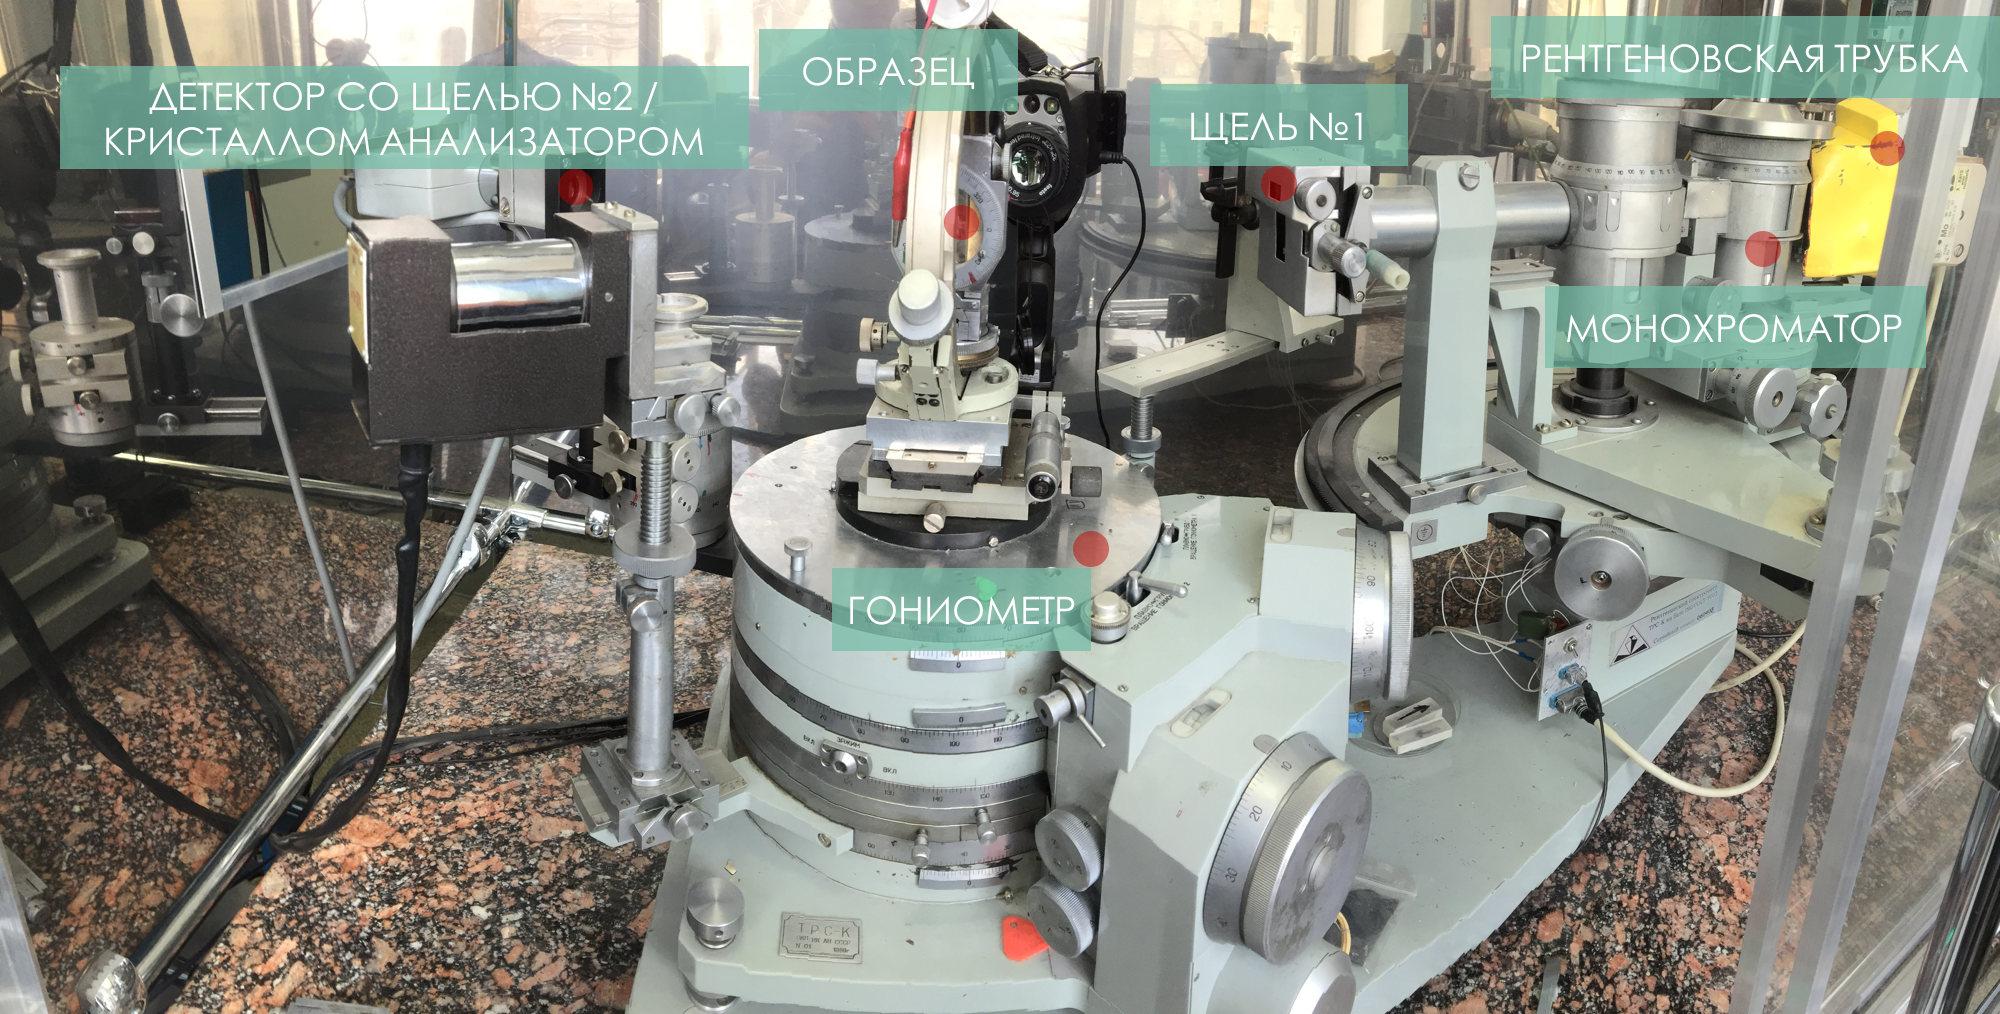
\includegraphics[width=1\textwidth]{images/trs.png}
  \caption{ Трехкристальный рентгеновский спектрометр. Лаборатория рентгеновских
  методов анализа и синхратронного излучения, ФНИЦ "Кристаллография и фотоника"}
  \label{ris:trs}
\end{figure}

ТРС имеет возможность работать в режиме двухкристального эксперимента,
в таком случае непосредственно перед детектором устанавливается щелевое устройство
№ 2, все прошедшие лучи фиксируются детектором.

Для случая необходимости получения трехкристальных кривых дифракционного отражения,
на место перед детектором устанавливается кристалл анализатор, отраженный от анализатора луч
фиксируется детектором.

\subsection{Функция источника}
Спектр рентгеновской трубки является характеристическим, спектральная часть
 которого достаточно хорошо описывается двумя функциями Лоренца взятыми с
 весовыми коэффициентами (\ref{eq:source_spectral}).

 \begin{equation} \label{eq:source_spectral}
   g_{\lambda} (\lambda) = \frac{2\pi}{3}  \left \{ \frac{\delta\lambda_1}{(\lambda - \lambda_1)^2+
   (\delta \lambda_1)^2} + \frac{1}{2} \frac{\delta\lambda_2}{(\lambda-\lambda_1)^2+(\delta\lambda_1)^2} \right \}
  \end{equation}

  Плотность распределения количества потока электромагнитного излучения в зависимости от угла
  отстройки относительно прямолинейного распределения задается функцией Гаусса \ref{eq:source_angle}.

  \begin{equation} \label{eq:source_angle}
    g_{\vartheta} (\vartheta) = \frac{1}{\sigma \sqrt{ 2\pi}} exp  ( -\frac{\vartheta^2}{2\sigma^2} )
   \end{equation}
где $\sigma$ - параметр, который характеризует ширину углового распределения на половине высоты.

\begin{figure}[H]
  \centering
  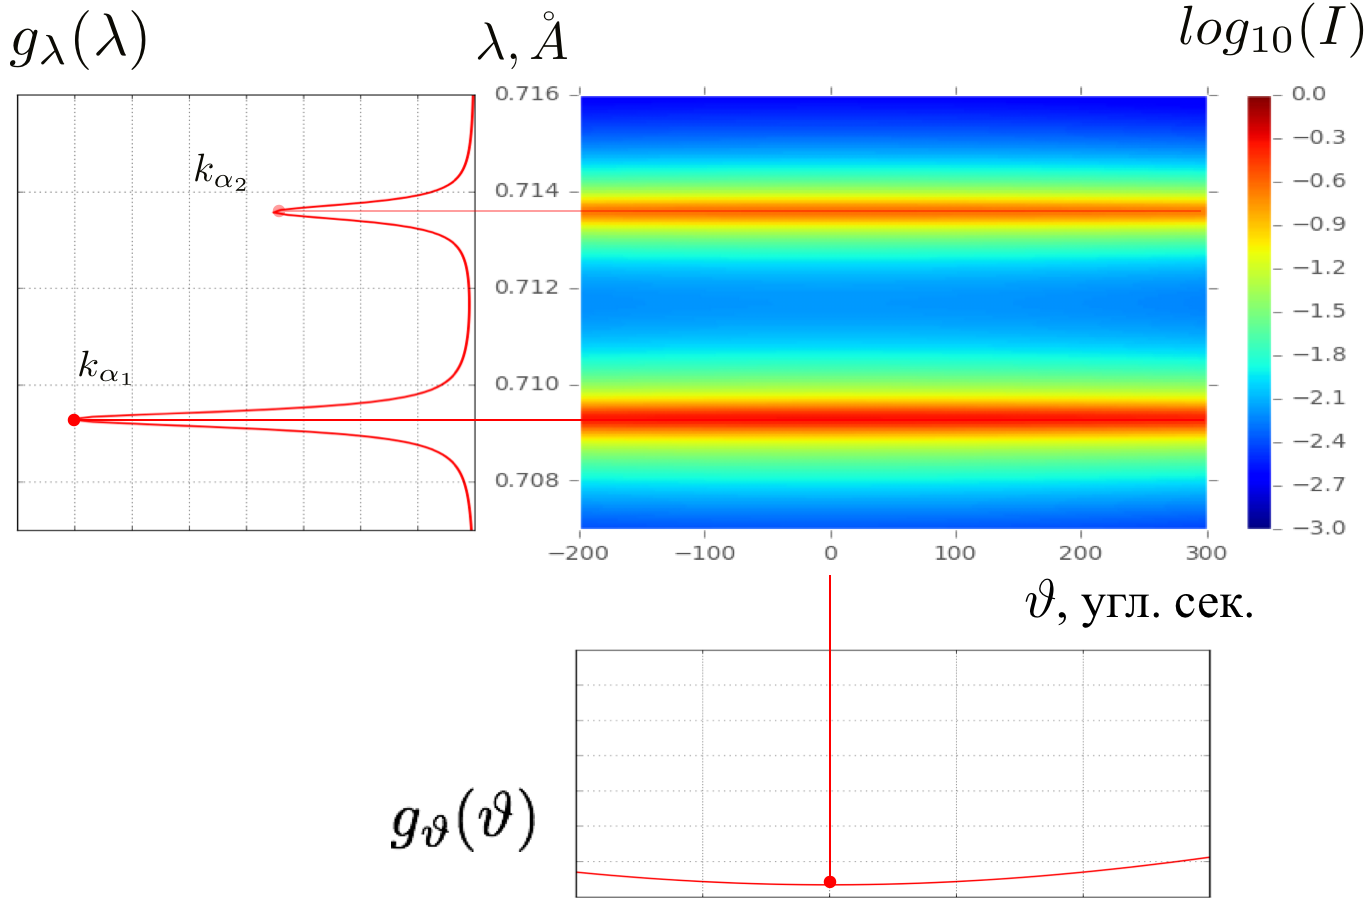
\includegraphics[width=0.6\textwidth]{images/source_distrubition.png}
  \caption{Спектрально – угловое распределение лабораторного источника рентгеновского
   излучения с молибденовым анодом, угловая полуширина распределения составляет $\sigma = 600$ угл. сек. }
  \label{ris:source_distrubition}
\end{figure}


 \subsection{Функция щелевых коллиматоров}
 Рассмотрим преобразование пучка рентгеновского излучения проходящего через систему щелевых коллиматоров.
 \begin{figure}[H]
   \centering
   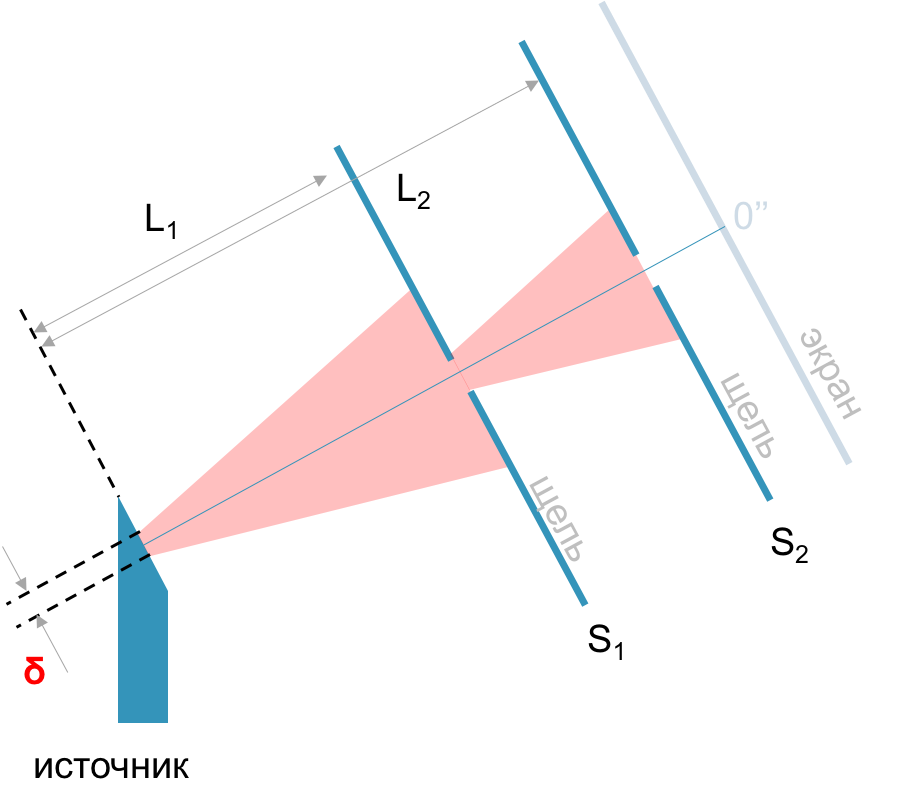
\includegraphics[width=0.6\textwidth]{images/for_slits.png}
   \caption{Схематичное представление щелевых устройств}
   \label{ris:for_slits}
 \end{figure}

На начальном этапе мы рассматривали модель точечного источника излучения $\delta = 0$.
В таком случае, интенсивность проходящего излучения будет определятся
одним щелевым устройством, которое является более узким в пересчете в угловые
координаты. Например, для фиксированных расстояний между элементами,
($L_1 = 570$ мм, $L_2 = 1005$ мм), в случае одинаковых линейных размеров щелей и точечного
источника, интенсивность будет определяться более удаленным щелевым устройством и
распределение интенсивности принимает вид ступеньки (рисунок ~\ref{ris:sourc_map_a}). Если источник является
 продолжительным $\delta \neq 0$, то угловое распределение интенсивности принимает более сложный вид, как показано на рисунке ~\ref{ris:sourc_map_b}.



 \begin{figure}[H]
   \centering
   \subfloat[Точечный источник]{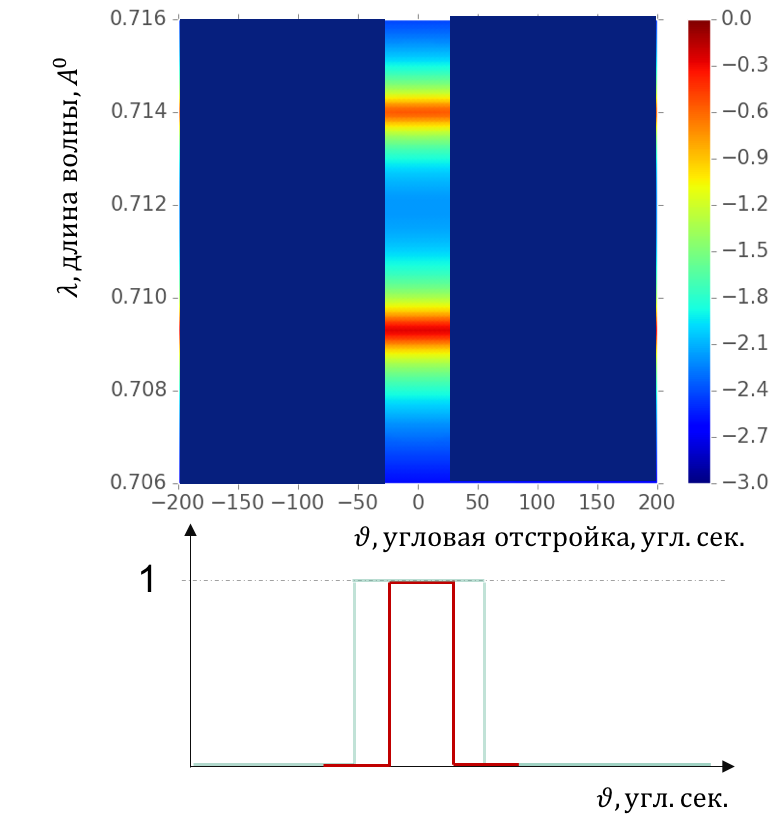
\includegraphics[width=0.5\textwidth]{images/point_sourc_map.png}\label{ris:sourc_map_a}}
   \hfill
   \subfloat[Источник с линейным размером $\delta = 0.2$ мм]{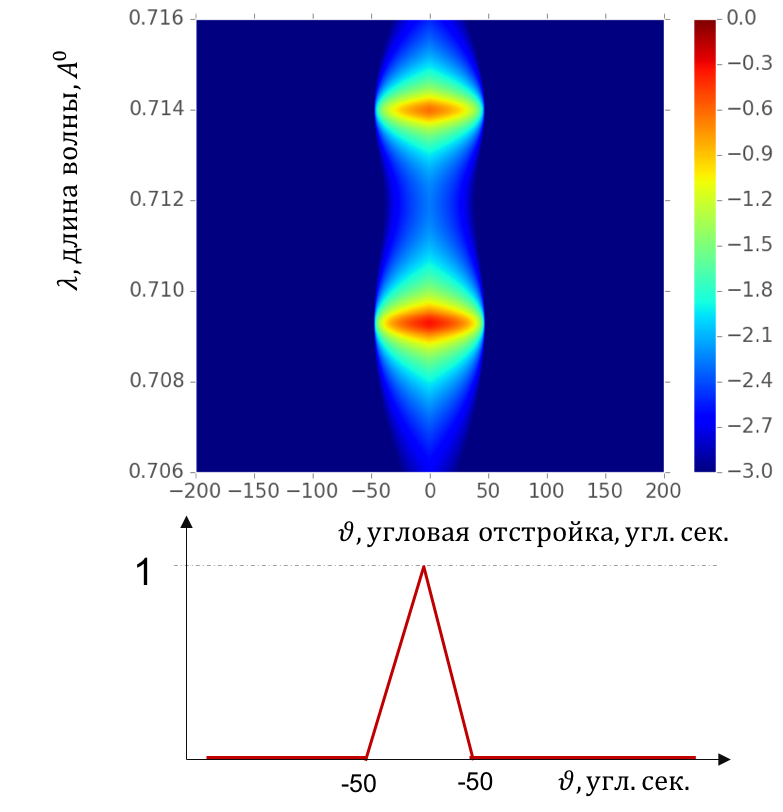
\includegraphics[width=0.5\textwidth]{images/wide_sourc_map.png}\label{ris:sourc_map_b}}
   \caption{Спектрально угловое распределение источника в система двух щелей}
   \label{ris:sourc_map}
 \end{figure}

 Необходимо отметить, что для описания дифракционного эксперимента важно расчитывать именно
 угловое распределение, т.е. знать количество и величину энергии квантов падающих под тем
 или иным углом на кристалл. Для того, чтобы это сделать нам необходимо посчитать площадь параллелограммов
 (рисунок \ref{ris:how_many_quants_use_parallelogr}),

 \begin{figure}[H]
   \centering
   \subfloat[Пропускная способность системы пропорциональна площади
   соответствующего параллелограмма ]{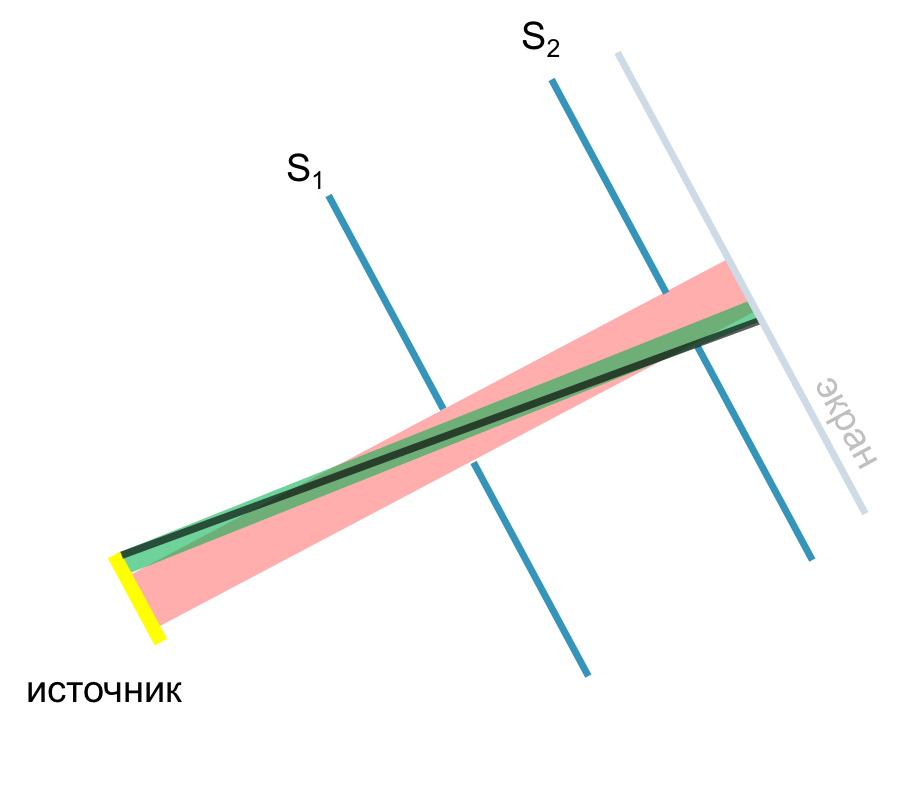
\includegraphics[width=0.45\textwidth]{images/how_many_quants_use_parallelogr_1.png}}
   \hfill
   \subfloat[Интенсивность на экране $\delta = 0.2$ мм]{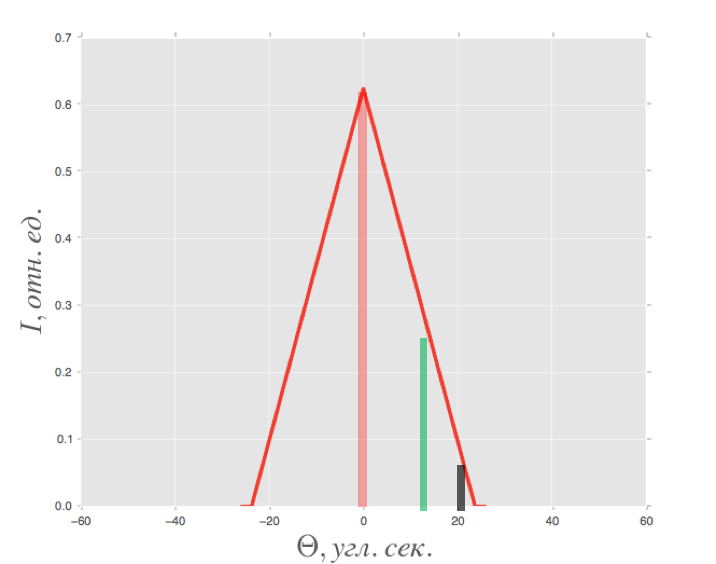
\includegraphics[width=0.45\textwidth]{images/how_many_quants_use_parallelogr_2.png}}
   \caption{Схематичное представление расчета интенсивности углового
   распределения излучения после прохождения системы щелевых коллиматоров}
   \label{ris:how_many_quants_use_parallelogr}
 \end{figure}
Более подробный расчет представлен в (\ref{sec:calc_slits_ability}).
На рисунке (\ref{ris:calc_slits_ability_res}) представлены результаты расчета пропускной способности системы двух щелей для некоторых параметров в
приближении точечного и продолжительного источника.

\begin{figure}[H]
  \centering
  \subfloat[$S_1 = S_2 = 50$ мкм; $\delta = 0.2$ мм;]{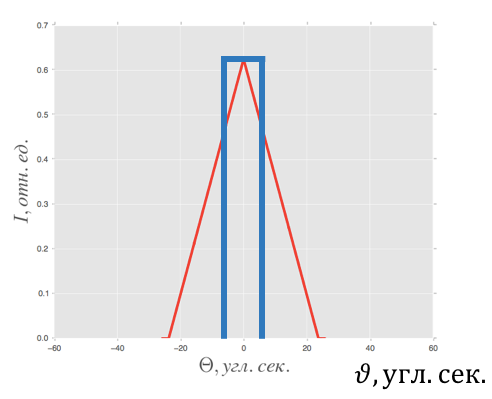
\includegraphics[height=6em]{images/calc_slits_ability_res_1.png}}
  \hfill
  \subfloat[$S_1 = 20$ мкм; $S_2 = 40$ мкм; $\delta = 0.2$ мм;]{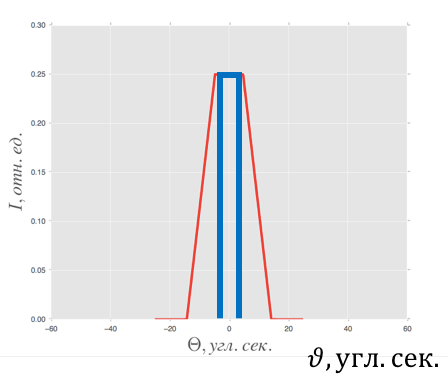
\includegraphics[height=6em]{images/calc_slits_ability_res_2.png}}
  \hfill
  \subfloat[$S_1 = 200$ мкм; $S_2 = 400$ мкм; $\delta = 0.2$ мм;]{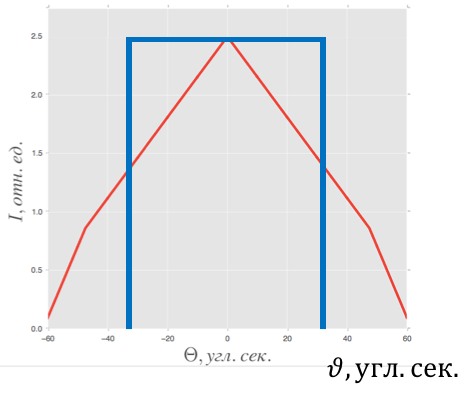
\includegraphics[height=6em]{images/calc_slits_ability_res_3.png}}
  \hfill
  \subfloat[$S_1 = 200$ мкм; $S_2 = 400$ мкм; $\delta = 0.1$ мм;]{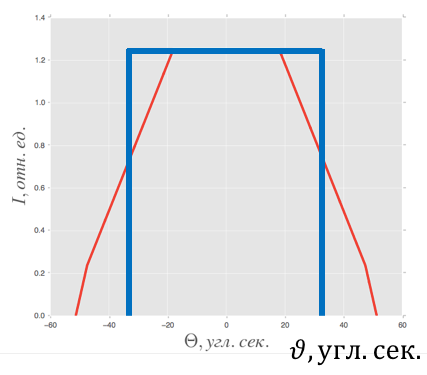
\includegraphics[height=6em]{images/calc_slits_ability_res_4.png}}
  \caption{$L_1 = 570$ мм; $L_2 = 1005 $ мм }
  \label{ris:calc_slits_ability_res}
\end{figure}

\subsubsection{Отражение от одного кристалла}
  Постепенно будем наполнять схему и внесем один идеальный кристаллический элемент.
  Кристалл регламентируется уже не только угловой составляющей пучка, но и берет в учет энергию.
\begin{figure}[H]
  \centering
  \subfloat[Схема однокристального эксперимента]{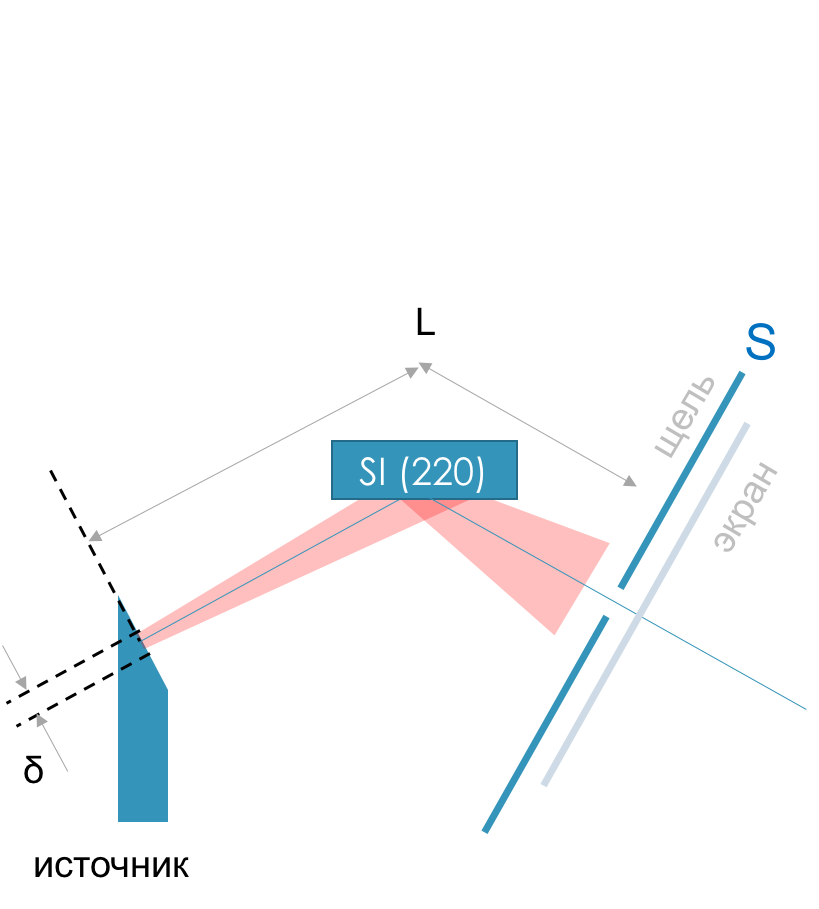
\includegraphics[width=0.45\textwidth]{images/single_crystal_schem.png}}
  \hfill
  \subfloat[Спектрально угловое распределение]{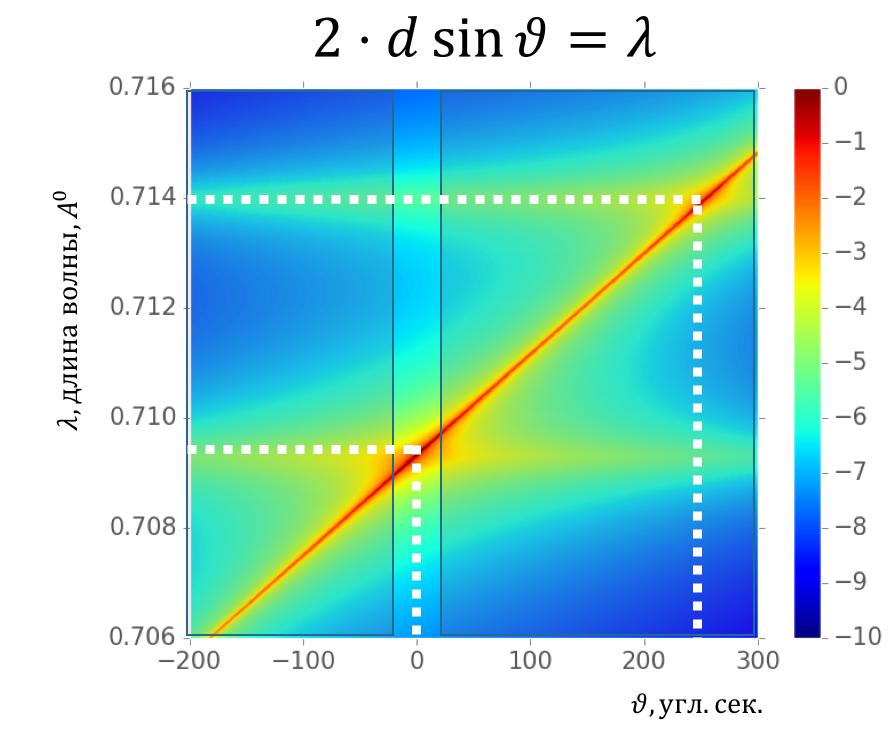
\includegraphics[width=0.45\textwidth]{images/single_crystal_schem_lamtet.png}}

  \caption{Спектрально угловое распределение после отражения расходящегося, полихромотического пучка от кристалла}
  \label{ris:single_crystal_schem_lamtet}
\end{figure}

На рисунке \ref{ris:single_crystal_schem_lamtet} изображен принцип работы монохроматора,
когда после взаимодействия с ним, разные длины волн отражаются под разными углами в
соответсвии с законом Брегга.

\begin{figure}[H]
  \centering
  \subfloat[$S = 50$ мкм; ]{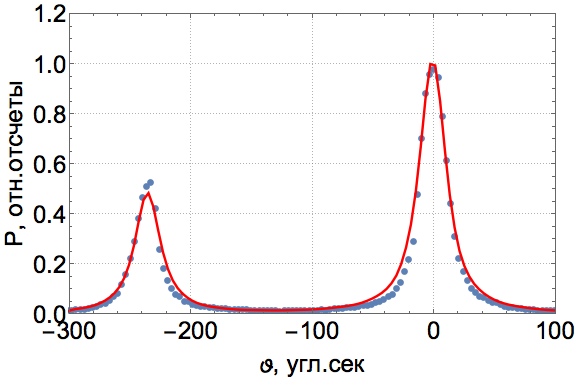
\includegraphics[width=0.7\textwidth]{images/single_cr_exp_s_005mm.png}}
  \hfill
  \subfloat[$S = 200$ мкм;]{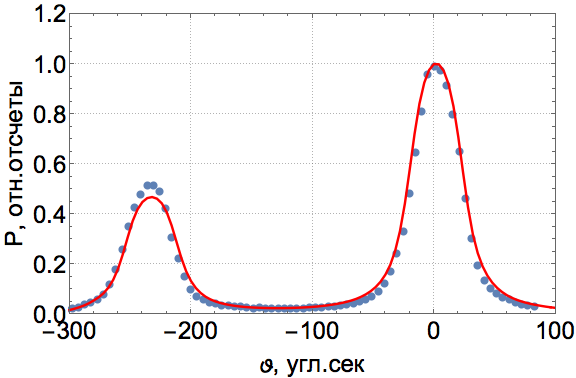
\includegraphics[width=0.7\textwidth]{images/single_cr_exp_s_02mm.png}}
  \caption{Однокристальный эксперимент}
  \label{ris:zero_exp}
\end{figure}


   \subsubsection{Дифракция на щели}
      Cowley1979ru на странице 47
  

Измерение кривой дифракционного отражения в двухкристальной схеме представляет
собой измерение зависимости отраженного образцом рентгеновского излучения при
пошаговом повороте исследуемого кристалла относительно падающего на него
излучения в окрестности точного значения угла Брэгга.
Существует несколько схем измерения кривых отражения рентгеновского излучения.

\subsubsection*{$\omega$ - сканирование}
В данном типе сканирования кривая отражения измеряется путем поворота образца
относительно падающего пучка в плоскости дифракции. При таком сканировании
угол между падающим и дифрагированным пучками (угол рассеяния) остается постоянным
(рисунок ~\ref{ris:omega_scan}). Получаемая в результате кривая носит название кривой качания.


\begin{figure}[H]
  \centering
  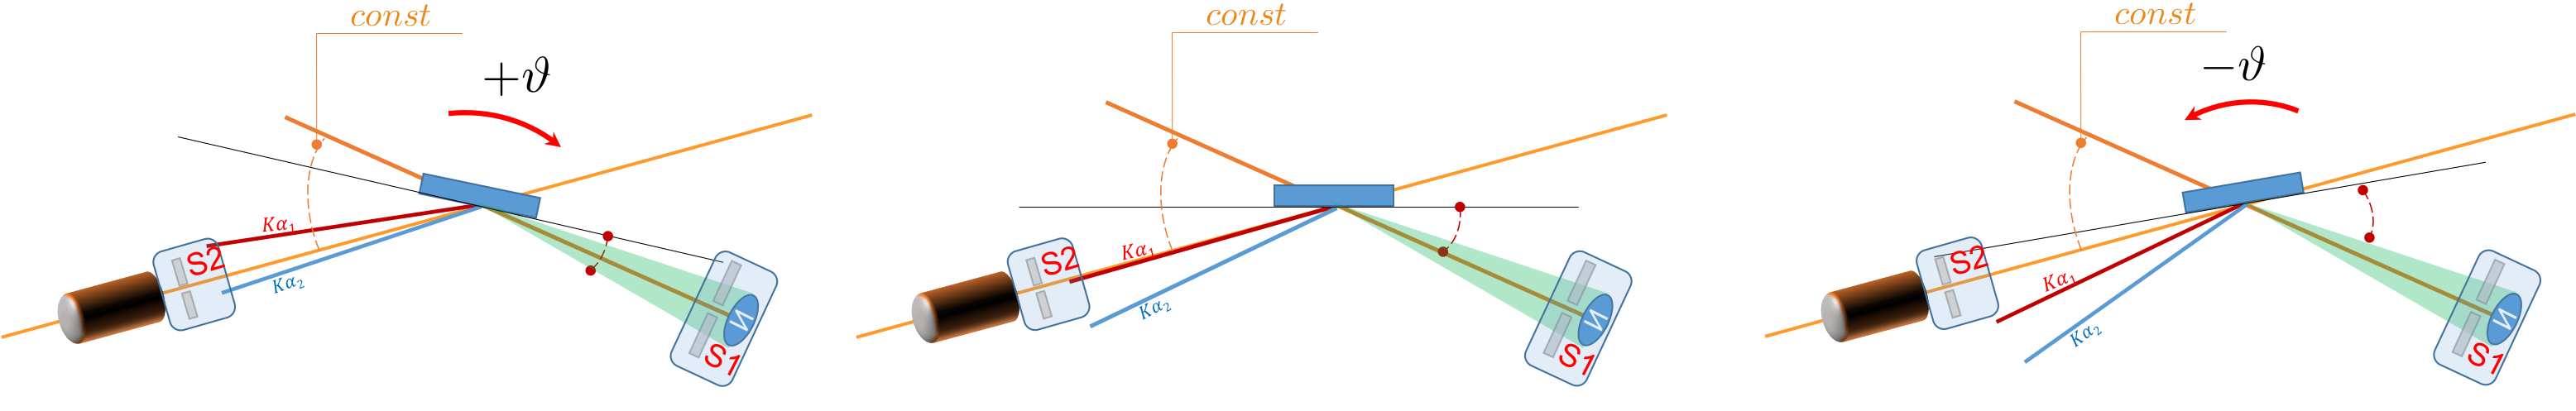
\includegraphics[width=1\textwidth]{images/omega_scan.png}
  \caption{Схема реализации $\omega $ - сканирования}
  \label{ris:omega_scan}
\end{figure}

\subsubsection*{$\vartheta - 2\vartheta$ - сканирование}
В отличие от предыдущего, данный метод сканирования соответствует изменению
 модуля вектора рассеяния при неизменном его угловом положении
 (рисунок ~\ref{ris:theta_2theta_scan}). Угловое положение падающего пучка и
 детектора изменяется синхронно и симметрично относительно используемой системы
 атомных плоскостей, а установленная перед детектором апертурная щель вырезает
  только зеркально отраженную часть пучка. Именно поэтому при построении карт
   пространственного распределения спектра полосы щелей на этих картах остаются
   неподвижными (т.к. несмотря на движение щели  $S_2$ в процессе
    $\vartheta - 2\vartheta$ -  сканирования ее отстройка от зеркального
    положения всегда равна 0).

 \begin{figure}[H]
   \centering
   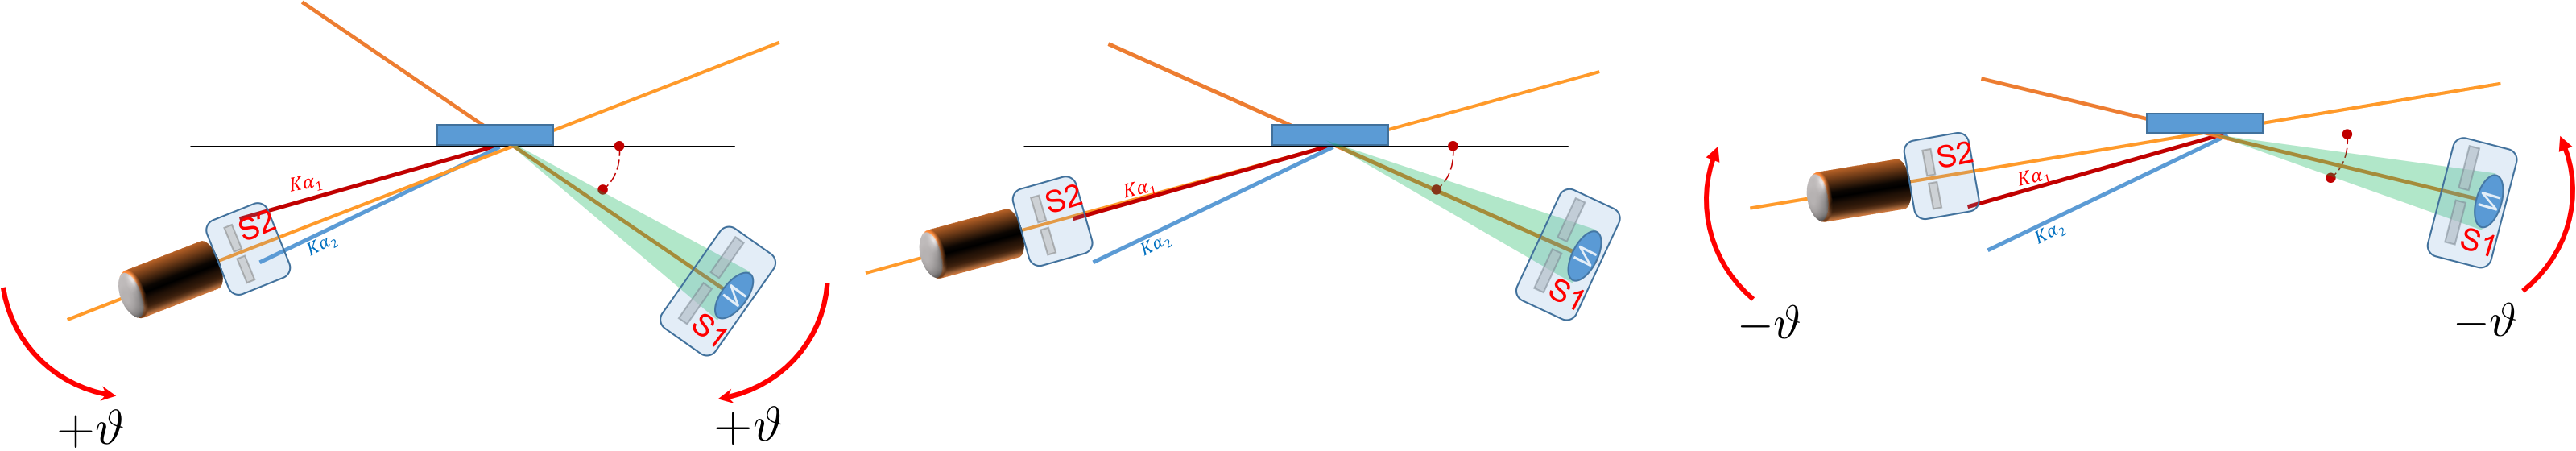
\includegraphics[width=1\textwidth]{images/theta_2theta_scan.png}
   \caption{Схема реализации $\vartheta - 2\vartheta$ - сканирования}
   \label{ris:theta_2theta_scan}
 \end{figure}
Кроме того, используемый подход позволяет наглядно продемонстрировать интересный эффект.
 Независимо от ширины входной и приемной щелей характеристическая линия спектра
 трубки $k_{\alpha 2}$ всегда вносит вклад в КДО, проявляясь в виде дополнительного
 пика на ее хвосте (рис. 2.21). Данный слабый пик возникает за счет того, что
 даже при очень малой входной щели $S_1$ линия $k_{\alpha 2}$ будет, отражаясь на «хвосте»
 кривой монохроматора, пролетать через входную щель и, при определённом угле
 поворота образца, интенсивно дифрагировать в максимуме его собственной кривой
 отражения и давать весомый ($~10^{-6}$) вклад в общую интенсивность КДО.


\subsection{Методика расчета пьзоэлектрических констант по данным дифракции}

\newpage
\section{Расчеты и эксперименты}
\subsection{Нолькристальный эксперимент}
\subsection{Однокристальный эксперимент}
\subsection{Двухкристальный эксперимент}


  
\label{sec:non_disspers_KDO_section}
На рис. \ref{ris:non_disspers_kdo} приведены бездисперсионные двухкристальные КДО, рассчитанные в соответсвии
с выражением (\ref{eq:doudle_spectra_angle_map_on_detector}). В качестве кристалла-монохроматора
и образца был выбран монокристалл кремния с системой отражающих плоскостей (220), эксперимент проводился в
соответсвии со схемой, представленной на рис. \ref{ris:double_crystal_schem_lamtet_a}.

\begin{figure}[H]
  \centering
  \subfloat[]{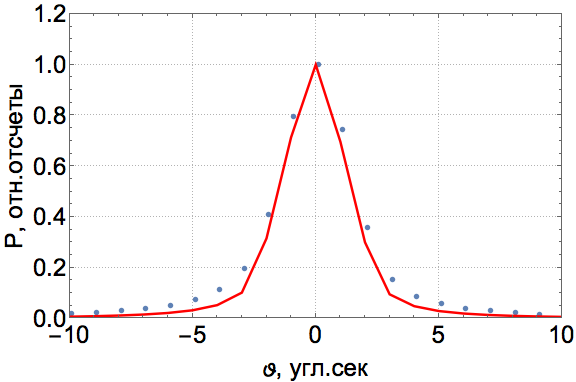
\includegraphics[width=0.45\textwidth]{images/non_disspers_20_40.png}\label{fig:f1}}
  \hfill
  \subfloat[]{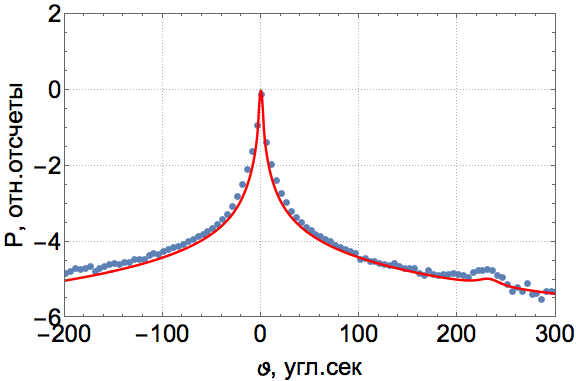
\includegraphics[width=0.45\textwidth]{images/non_disspers_20_40_log.png}\label{fig:non_disspers_kdo_1}}
  \hfill
  \subfloat[]{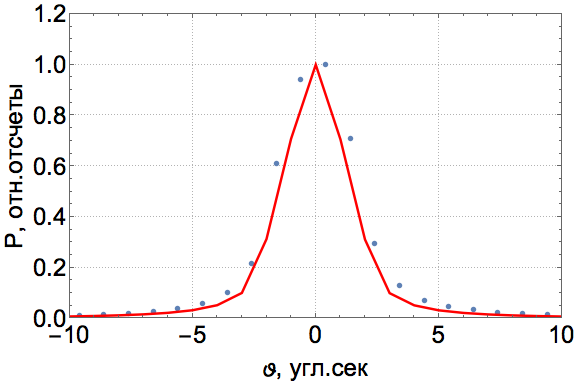
\includegraphics[width=0.45\textwidth]{images/non_disspers_300_200.png}\label{fig:f2}}
  \hfill
  \subfloat[]{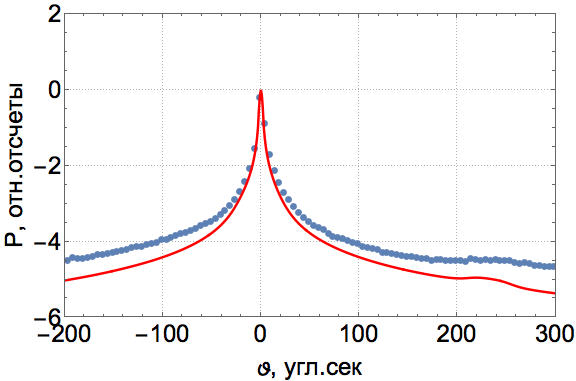
\includegraphics[width=0.45\textwidth]{images/non_disspers_300_200_log.png}\label{fig:f2}}
  \caption{Двухкристальная бездисперсионная КДО для схемы с установленными
   кристаллом-монохроматором Si(220) и образцом Si(220). Расстояние до щелевых коллиматоров
  составляет $L_1= 570 $мм, $L_2 = 1005$ мм соответсвенно.
  Линейный размер источника $\delta = 0.1$ мм. Расчет - (красная линия), эксперимент - (синие точки).
  Результаты приведены для размеров щелевых коллиматоров  $S_1 = 20 $ мкм; $ S_2 = 40$ мкм (a),
    $S_1 = 20 $ мкм; $ S_2 = 40$ мкм (b),
   $S_1 = 300 $ мкм; $ S_2 = 200$ мкм (c),
    $S_1 = 300 $ мкм; $ S_2 = 200$ мкм (d)}
  \label{ris:non_disspers_kdo}
\end{figure}

На рис. \ref{fig:non_disspers_kdo_1} видно, что наряду с главным пиком, соответствующим $K_{\alpha1}$ - линии
излучения, на которую настроен монохроматор, присутствует вклад от соседней характеристической линии
 $K_{\alpha2}$. Впервые, на это свойство двухкристальных КДО, получаемых в бездисперсионной
схеме в случае использования рентгеновской трубки было указано авторами работы \cite{chuev2008}.

\begin{figure}[H]
  \centering
  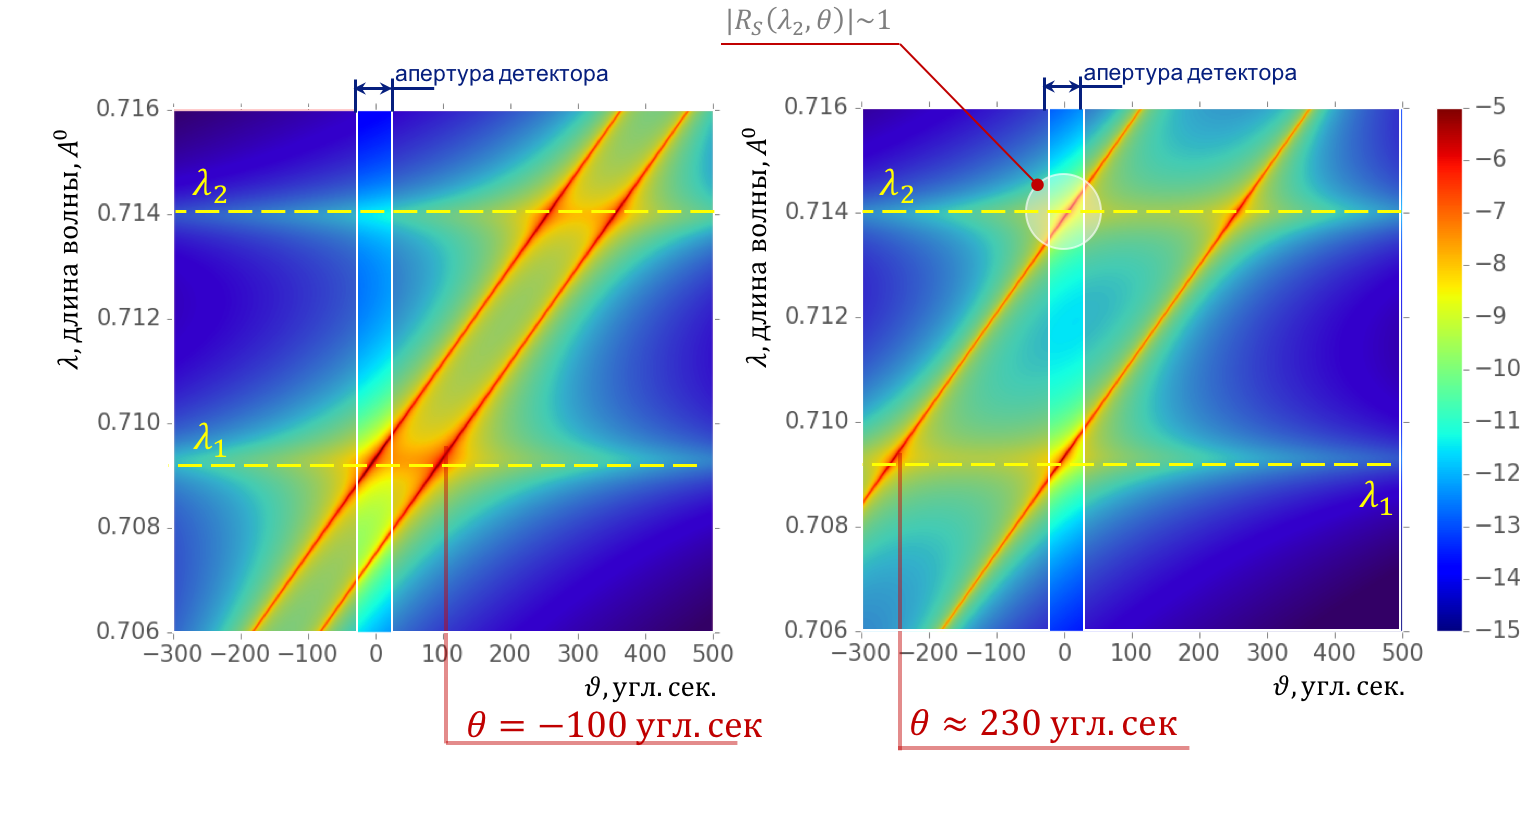
\includegraphics[width=0.8\textwidth]{images/vklad_kalpha2.png}
  \caption{Схематичное объяснение эффекта образования дополнительного пика на двухкристальных КДО
  с помощью спектрально-углового представления}
  \label{ris:vklad_kalpha2}
\end{figure}

На рис. \ref{ris:vklad_kalpha2} наглядно изображен механизм формирования дополнительного пика,
соответствующего $K_{\alpha 2}$ - составляющей спектра. В точке образования пика ($\theta = 230$ угл.сек.), коэффициент
отражения  (см. \ref{eq:doudle_spectra_angle_map_on_detector})
для кристалла образца при длине волны $\lambda_2$ максимален (в случае кристалла Si равен 1). Но отражение
от монохроматора в этой точке является слабым, т.о. интенсивность дополнительного пика на 5 порядков меньше
интенсивности основного, в отличие когда реализуется сильное отражение от обоих кристаллов.
 Необходимо отметить, что пик фактически существует вне зависимости от размера щелевых коллиматоров, но
при достаточно больших размерах (200 мкм.) пропадает на фоне хвостов КДО $K{\alpha 1}$ - линии.

  \subsubsection{Дисперсионная схема дифракции}
  Дисперсия возникает когда есть некое спектральное распределение источника и
   угол Брегга монохроматора отличается от угла Брегга исследуемого кристалла-образца
   (рисунок \ref{fig:double_crystal_schem_disp_a}).
   коэффициентом отражения.
  \begin{figure}[H]
    \centering
    \subfloat[$\theta_B^M \neq \theta_B^S$]{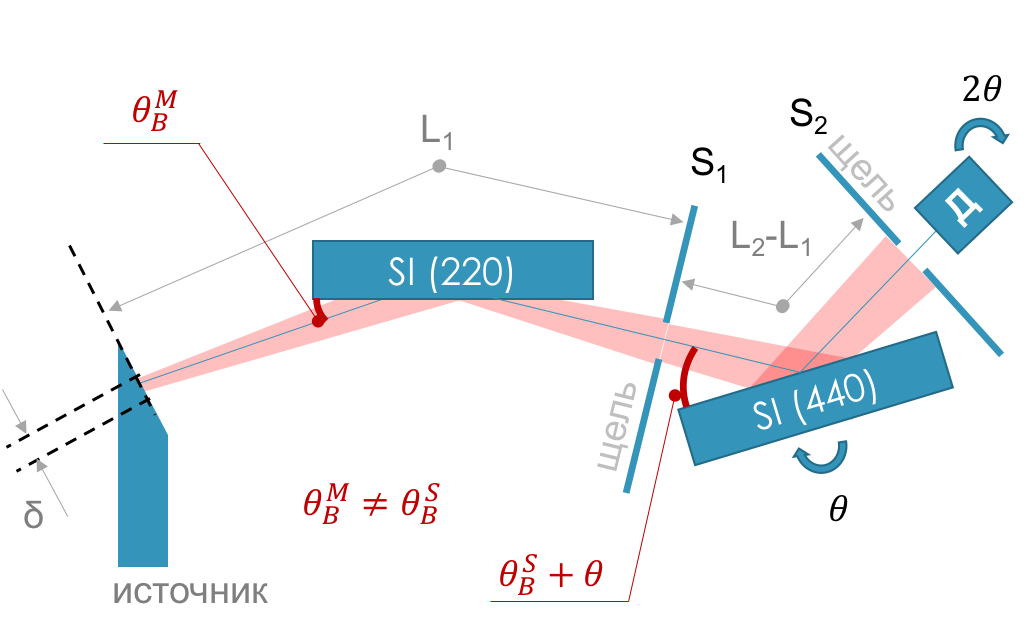
\includegraphics[width=0.6\textwidth]{images/double_crystal_schem_disp.png}\label{fig:double_crystal_schem_disp_a}}
    \hfill
    \subfloat[Спектральное-угловое распределение]{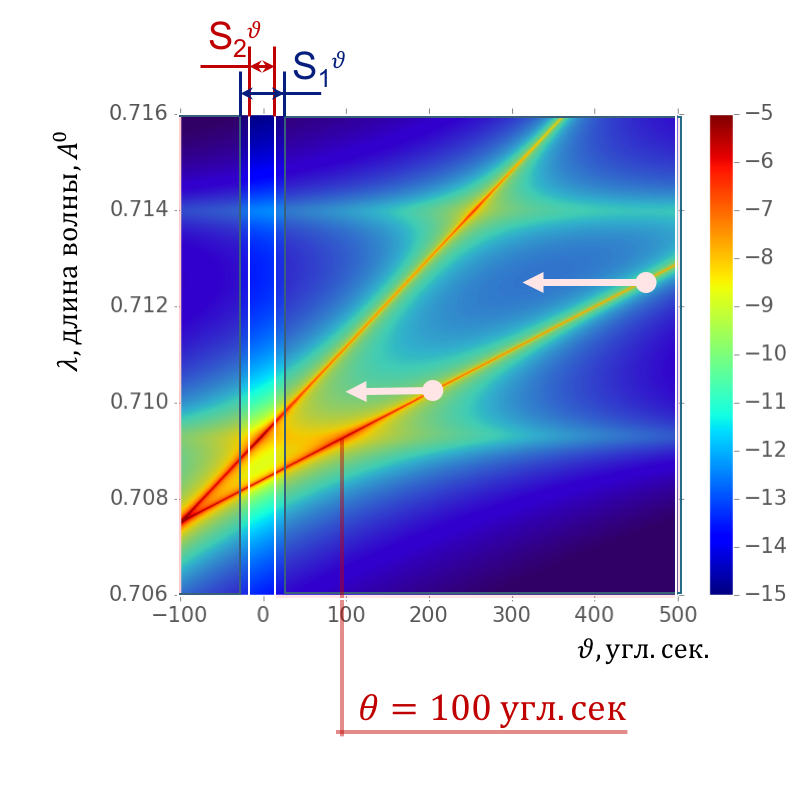
\includegraphics[width=0.35\textwidth]{images/double_crystal_lamtet_disp.png}\label{fig:double_crystal_schem_disp_b}}
    \caption{Дисперсионная схема дифракции}
    \label{ris:double_crystal_schem_disp}
  \end{figure}
  Факт наличия дисперсии возможно проанализировать на спектрально-угловом распределении
  (рисунок \ref{fig:double_crystal_schem_disp_b}), прямая образца в этом случае не параллельна прямой монохроматора и
  в области близкой к точному брегговскому отражению происходит не наложение одной на другую, как в случае отсутствия дисперсии,
  а пересечение. В точке пересечение коэффициент отражения практически равен единице,
  легко заметить что кривая отражения будет уширенной (рисунок \ref{ris:disspersion_curves_expantheory}).
\begin{figure}[H]
  \centering
  \subfloat[Образец Si(440) - $\theta_B = 21.7^o$, $S_1 = S_2 = 100$ мкм.]{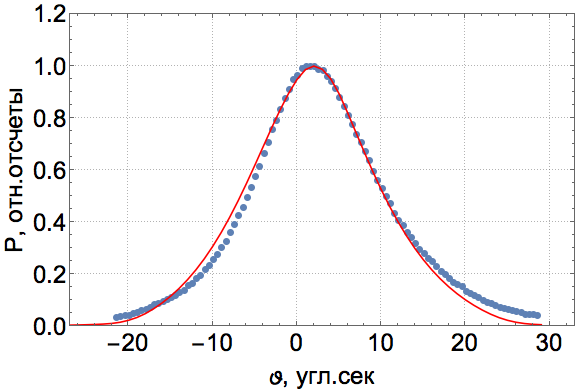
\includegraphics[width=0.45\textwidth]{images/disspers_220_440_100mcm.png}\label{fig:}}
  \hfill
  \subfloat[Образец Si(660) - $\theta_B = 33.7^o$, $S_1 = S_2 = 100$ мкм.]{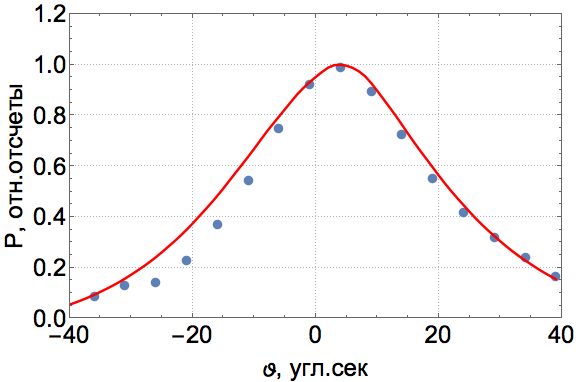
\includegraphics[width=0.45\textwidth]{images/disspers_220_660_100mcm.png}\label{fig:}}
  \hfill
  \subfloat[Образец Si(440) - $\theta_B = 21.7^o$, $S_1 = S_2 = 300$ мкм.]{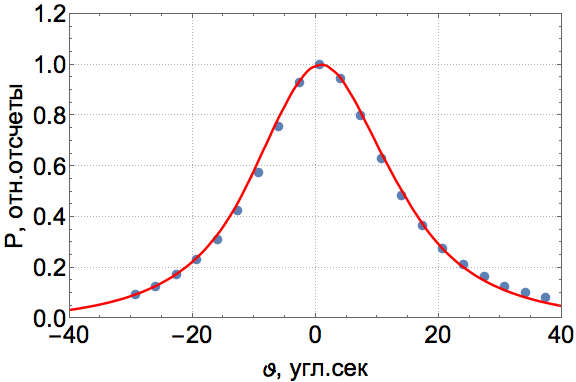
\includegraphics[width=0.45\textwidth]{images/disspers_220_440_300mcm.png}\label{fig:}}
  \hfill
  \subfloat[Образец Si(660) - $\theta_B = 33.7^o$, $S_1 = S_2 = 300$ мкм.]{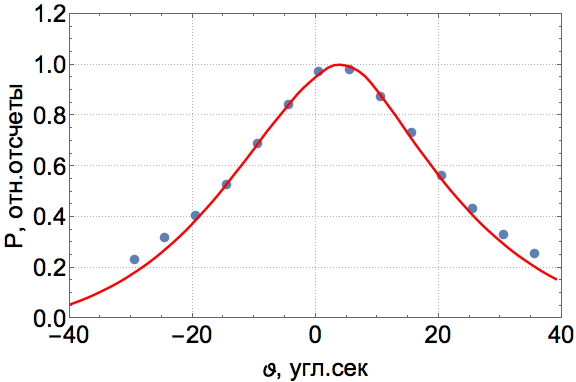
\includegraphics[width=0.45\textwidth]{images/disspers_220_660_300mcm.png}\label{fig:}}
  \caption{Двухкристальная КДО для схемы с кристаллом монохроматором Si(220) - $\theta_B = 10.6^o$ для дисперсионного случая для разных размеров щелевых устройств}
  \label{ris:disspersion_curves_expantheory}
\end{figure}

 В отличие от бездисперсионных КДО (раздел \ref{sec:non_disspers_KDO_section}) заметно присутствует
 влияние размера щелевых устройств.

    \subsubsection{Асимметричная схема дифракции}


  \begin{figure}[H]
    \centering
    \subfloat[$b = 33.52$, $\varphi$ > 0]{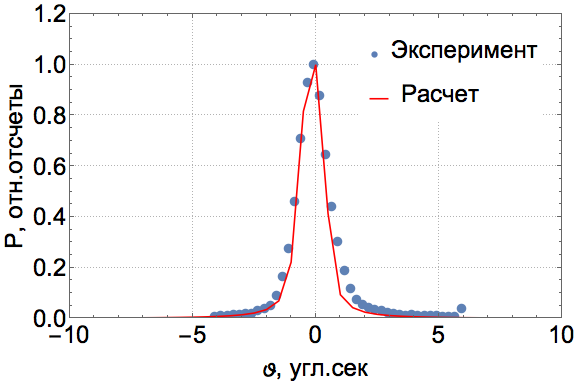
\includegraphics[width=0.45\textwidth]{images/assym-blue-50.png}}
    \hfill
    \subfloat[$b = 0.03$, $\varphi$ < 0]{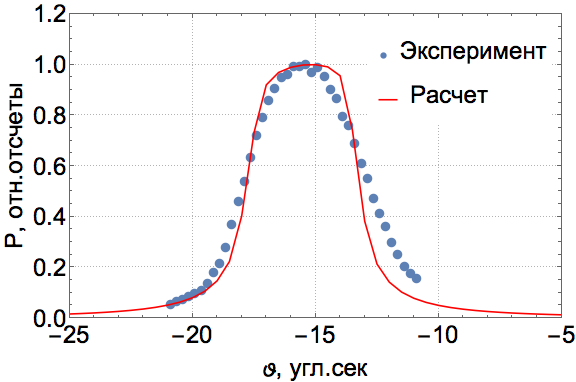
\includegraphics[width=0.45\textwidth]{images/assym-red-50.png}}
    \caption{Двухкристальная КДО для схемы с кристаллом монохроматором Si(440) и асимметричным образцом Si(440),
    угол разориентации поверхности $\varphi = 20^o53^{'}$. Размер щелевых устройств $S_1 = S_2 = 50$ мкм.}
    \label{ris:assymetric_exp_50}
  \end{figure}





\newpage
\begin{center}
\begin{thebibliography}{99}

\bibitem{International_Tables}
  P. J. Brown, A. G. Fox, E. N. Maslen, M. A. O'Keefe and B. T. M. Willis.
  International Tables for Crystallography (2006). Vol. C, ch. 6.1, pp. 554-595
\bibitem{f0f1f12}
J. Coraux, V. Favre-Nicolin, M. G. Proietti et al. // Phys.Rev. B. – 2007. – 75. – 235312

\bibitem{afanasyev1989}
  А. М. Афанасьев, П. А. Александров, Р. М. Имамов. Ренгеновская диагностика
  субмикронных слоев. - Москва: Наука, 1989 г. - 152 с.

\bibitem{pinsker1982}
  З. Г.  Пинскер. Рентгеновская кристаллооптика. - Москва: Наука, 1982 г. - 292 с.

  \bibitem{iveronova1972}
    В. И.  Иверонова, Г. П. Ревкевич. Теория рассеяния ренгеновских лучей. -
    Москва: Издательство московского университета, 1972 г. - 248 с.
\bibitem{Willis1975}
  Willis, B. T. M. Thermal vibrations in crystallography /
  B. T. M. Willis, A. W. Pryor. — Cambridge University Press, 1975. —P. 279.

\bibitem{kibalin2015}
  Ю. А. Кибалин. Диффракционные исследования атомных колебаний в легкосплавных
  металлах, наноструктуррированных внутри пористых сред. [Текст]: автореф. дис. на соиск.
   учен. степ. канд. физ. - мат. наук (01.04.07) /
   Кибалин Юрий Андреевич; НИЦ "Курчатовский институт". – Москва, 2015. – 99 с.

\bibitem{fetisov2007}
  Г. В. Фетисов. Синхротронное излучение. Методы исследования структуры веществ. -
  Москва: ФИЗМАТЛИТ, 2007 г. - 672 с. ISBN 978-5-9221-0805-8.

\bibitem{landau_8_1992}
 Л.Д. Ландау, Е.М. Лифшиц. Теоретическая физика. том 8 –
 Электродинамика сплошных сред, 2-е изд., Москва: Наука, 1992. - 661 с.
 \bibitem{Bushuev_Oreshko_2002}
 В. А. Бушуев, А. П. Орешко. зеркальное отражение рентгеновских лучей в условиях скользящей дифракции.
 Учебное пособие. Москва: МГУ, физический факультет, 2002. - 57 с.
 \bibitem{Tanner_1998}
 D. Keith Bowen, Brain K. Tanner. High Resolution X-Ray Diffractometry and Topography. - United Kingdom: Taylor and Francis, 1998. - 265 p.

\end{thebibliography}
% \cite{Tanner_1998}

\end{center}
\newpage
\appendix
\begin{center}
  \section{}%Выражение для поляризуемости}
\end{center}

\label{sec:polarizability}
% ~\ref{sec:wave_equation}
Приведем упрощенный вывод для Фурье компонент  $\chi_h$  для рентгеновской
поляризуемости в среде  $\chi(\vec{r})$. Если в какой либо точке находится электрон,
то уравнение его движения под действием электромагнитной волны,
исходя из второго закона Ньютона, запишется в виде \cite{iveronova1972}.
\begin{equation}
  \ddot{x}+ k\dot{x} + \omega_0^2 x = \frac{e}{m}E_0e^{i\omega t}
 \end{equation}
Откуда смещение этого заряда
\begin{equation}
  x = \frac{e}{m} \frac{E_0e^{i\omega t}}{\omega_0^2 - \omega^2+i\omega t}
 \end{equation}
где $\omega_0 $ - собственная частота колебания электрона (частота электронного перехода), $\omega$ - частота рентгеновского излучения.

Поляризация единицы объема в заданной точке пространства $P$ определяется из условия
$P = \frac{\sum e x}{\Delta V}$. Суммирование проводится по всем зарядам в
некотором малом объеме  $\Delta V$.

Для рентгеновских лучей обычно $\omega_0^2 << \omega^2$, поэтому
\begin{equation}
  4\pi P = - \frac{4\pi e^2}{m\omega^2}\frac{\Delta N}{\Delta V} E_0 e^{i\omega t} = -\frac{e^2 \lambda^2}{m \pi c^2} \rho E_0 e^{i\omega t}
 \end{equation}
где $\Delta N$ - число зарядов в объеме $\Delta V$;
$\rho = \frac{\Delta N}{\Delta V}$ - электронная плотность в заданной точке пространства.


\begin{equation}
  \chi_h = -\frac{e^2 \lambda^2}{m \pi c^2}  \rho = -\frac{e^2 \lambda^2}{m \pi c^2} \frac{F_h}{V}
 \end{equation}
 где, $ F_h = \sum_{n} f_n \cdot e^{-2\pi i\vec{h}\cdot \vec{r}_n}= \sum_{n} f_n \cdot e^{- 2 \pi i (hx_n+ky_n+lz_n)}$ -
 структурная амплитуда (раздел ~\ref{sec:structure_factor}),
 коэффициент $h$ в $F_h$ - означает конкретные значения индексов {hkl}; $V$ - объем элементарной ячейки кристалла.

\newpage
\begin{center}
\section{}%Волновое уравнение
\end{center}

 \label{sec:wave_equation}
  воспользоваться операторным тождеством
 \begin{equation}
   rot \quad rot \vec{E} = grad \quad div \vec{E} - \Laplace \vec{E}
  \end{equation}


% \begin{lstlisting}[language=Python]
% import numpy as np
%
% def incmatrix(genl1,genl2):
%     m = len(genl1)
%     n = len(genl2)
%     M = None #to become the incidence matrix
%     VT = np.zeros((n*m,1), int)  #dummy русский
%
%     #compute the bitwise xor matrix
%     M1 = bitxormatrix(genl1)
%     M2 = np.triu(bitxormatrix(genl2),1)
%
%     for i in range(m-1):
%         for j in range(i+1, m):
%             [r,c] = np.where(M2 == M1[i,j])
%             for k in range(len(r)):
%                 VT[(i)*n + r[k]] = 1;
%                 VT[(i)*n + c[k]] = 1;
%                 VT[(j)*n + r[k]] = 1;
%                 VT[(j)*n + c[k]] = 1;
%
%                 if M is None:
%                     M = np.copy(VT)
%                 else:
%                     M = np.concatenate((M, VT), 1)
%
%                 VT = np.zeros((n*m,1), int)
%
%     return M
% \end{lstlisting}


\end{document}
